% %
% This file is encoded in utf-8
% This file is modified from
% 1. http://exciton.eo.yzu.edu.tw/~lab/latex/latex_note.html
%    (元智大學模版 陳念波老師)
% 2. http://code.google.com/p/ntuthesis/
%    (臺大碩士、博士論文的Latex模板)
%%
\documentclass[12pt,a4paper]{ncku_class}

\usepackage{CJKutf8}  %%% ZZZ %%% macro for Chinese/Japanese/Korean processing
\usepackage{CJKnumb} %%% ZZZ %%% for Chinese numbering capability
\usepackage[nospace]{cite}  % for smart citation
\usepackage{geometry}  % for easy margin settings
\usepackage{ncku_style} % 自定義nckuee.sty // cbj


% 插圖套件 graphicx
% 使用者工作流程是用 pdftex 還是 latex + dvipdfmx?
% 視情況而有不同的參數
% 這裡作自動判斷
% 參考自
% http://www.tex.ac.uk/cgi-bin/texfaq2html?label=ifpdf
%%\newcommand\mydvipdfmxflow{dvipdfmx}P
%%\newcommand\mypdftexflow{pdftex}P
%%\ifx\pdfoutput\undefined
%%  % not running pdftex
%%  \usepackage[dvipdfm]{graphicx}
%%  \newcommand\myworkflow{dvipdfmx}  % set the flag for hyperref
%%\else
%%  \ifx\pdfoutput\relax
%%    % not running pdftex
%%    \usepackage[dvipdfm]{graphicx}
%%    \newcommand\myworkflow{dvipdfmx}  % set the flag
%%  \else
%%    % running pdftex, with...
%%    \ifnum\pdfoutput>0
%%      % ... PDF output
%%      \usepackage[pdftex]{graphicx}
%%      \newcommand\myworkflow{pdftex}  % set the flag
%%    \else
%%      %...DVI output
%%      \usepackage[dvipdfm]{graphicx}
%%      \newcommand\myworkflow{dvipdfmx}  % set the flag
%%    \fi
%%  \fi
%%\fi
      \usepackage[pdftex]{graphicx}
      \newcommand\myworkflow{pdftex}  % set the flag

% 增強功能型頁楣 / 頁腳套件
\usepackage{fancyhdr}  % 借用此套件來擺放浮水印
% (佔用了 central header)
% 不需要浮水印的使用者仍可利用此套件,產生所需的 header, footer
%
% 啟動 fancy header/footer 套件
\pagestyle{fancy}
\fancyhead{}  % reset left, central, right header to empty
\fancyfoot[C]{\thepage} %中間 footer 擺放頁碼
\renewcommand{\headrulewidth}{0pt} % header 的直線; 0pt 則無線

% 如果不需要任何浮水印,則請把下列介於 >>> 與 <<< 之間
% 的文字行關掉 (行首加上百分號)
%% 浮水印 >>>
%%%
% this file is encoded in utf-8
% v2.0 (Apr. 5, 2009)
% 如果浮水印不是全篇需要,請把下列介於 >>> 與 <<<
% 的「全篇浮水印專用碼」關掉 (行首加百分號)
% 參考自 Keith Reckdahl 寫的 "Using Imported Graphics in LATEX2e" (epslatex.pdf) p.39
% 如果只有特定頁需要浮水印
% 則依該頁屬性使用下列之一的命令 
% 普通頁命令 \thispagestyle{WaterMarkPage}
% plain 頁命令 \thispagestyle{PlainWaterMarkPage}
% empty 頁命令 \thispagestyle{EmptyWaterMarkPage}


% 將重複使用的浮水印章
% 圖檔是 my_watermark.xxx
% 副檔名可以不加,可以是 latex 系統能處裡的任何格式:pdf, gif, png, jpg, eps, ...
% 某些圖檔格式在某些工作流程可能需要作前置處裡。
% 例如,pdflatex 無法直接處理 eps 檔
%  latex + dvipdfmx 無法直接處理 pdf, gif, png, jpg, 需要用 ebb 小工具程式
%  對圖檔產生 .bb 對應檔。
%
% 寬為 5.1 cm
\newsavebox{\mywatermark}
%\sbox{\mywatermark}{
\includegraphics[keepaspectratio,%
%width=5.1cm]{ncku_watermark}} % // ncku_watermark.jpg 浮水印 // cbj

\sbox{\mywatermark}{
\includegraphics{header/ncku_watermark.jpg}
} % // ncku_watermark.jpg 浮水印 // Hong-Je

% 將 central header 擺放浮水印的巨集指令
\newcommand{\PlaceWaterMark}{\fancyhead[C]{\setlength{\unitlength}{1in}%
\begin{picture}(0,0)%
%\put(-1,-6.2){\usebox{\mywatermark}}% 圖檔擺放的位置座標
\put(-1.35,-6.55){\usebox{\mywatermark}}% 圖檔擺放的位置座標
\end{picture}}%
}

\fancyhead{}  % reset left, central, right header to empty
%% 如果不需整篇論文都要浮水印
%% 則下面  >>> 與 <<< 之間的程式碼請關閉
%% >>> 全篇浮水印
\PlaceWaterMark  % 每一頁都有浮水印 (除了 plain、empty 頁以外)

% 重新定義 plain 頁面
% 每張 plain 頁面 (每一章的第一頁) 也加浮水印

\fancypagestyle{plain}{%
\fancyhead{}%
\PlaceWaterMark%
\fancyfoot{}%
\fancyfoot[C]{\thepage}
\renewcommand{\headrulewidth}{0pt}%
\renewcommand{\footrulewidth}{0pt}%
}
%% <<< 全篇浮水印

%% 如果只有一、兩頁需要有浮水印
%% 可以在該頁 (有頁碼) 使用 \thispagestyle{WaterMarkPage}
%% 此命令不影響原有的 header、footer
\fancypagestyle{WaterMarkPage}{%
\PlaceWaterMark%
}

%% 如果只有一、兩頁 plain 頁需要有浮水印 (如 摘要、自傳等)
%% 可以在該頁 (有頁碼) 使用 \thispagestyle{PlainWaterMarkPage}
%% 只有頁碼與浮水印,沒有其他的 header、footer
%% 等同於 plain page style + water mark
\fancypagestyle{PlainWaterMarkPage}{%
\fancyhead{}%
\PlaceWaterMark%
\fancyfoot{}%
\fancyfoot[C]{\thepage}
\renewcommand{\headrulewidth}{0pt}%
\renewcommand{\footrulewidth}{0pt}%
}

%% 如果只有一、兩頁 empty 頁需要有浮水印 (如封面、書名頁)
%% 可以在該頁 (無頁碼) 使用 \thispagestyle{EmptyWaterMarkPage}
%% 等同於 empty page style + water mark
\fancypagestyle{EmptyWaterMarkPage}{%
\fancyhead{}%
\PlaceWaterMark%
\fancyfoot{}%
\renewcommand{\headrulewidth}{0pt}%
\renewcommand{\footrulewidth}{0pt}%
}

%% <<< 浮水印
% 如需額外的頁楣 (header) 或 footer,請在 header/header_footer.tex 裡依例修改
% 它的預設內容是都關掉,可依需要打開
%
% this file is encoded in utf-8
% v2.0 (Apr. 5, 2009)

%%%%%%% 其他的 header (left, right) 定義
% 底下定義了一些常見的 header 型式
% 預設情況是關掉的
% 使用者可以視需要將之打開
% 也就是把下列介於 >>> 與 <<< 之間
% 的文字行打開 (行首去掉百分號)

%% header >>>
%\renewcommand{\chaptermark}[1]{%
%\markboth{\prechaptername\ \thechapter\ \postchaptername%
%\ #1}{}%
%}  %定義 header 使用的「章」層級的戳記
%\fancyhead[L]{} % 左 header 為空
%\fancyhead[R]{\leftmark}  % 右 header 擺放「章」層級的戳記 (以 \leftmark 叫出)
%\renewcommand{\headrulewidth}{0.4pt}  % header 的直線 0.4pt; 0pt 則無線
%% <<< header

%%%%%%% 其他的 footer (left, right) 定義
% 底下定義了一些常見的 footer 型式
% 預設情況是關掉的
% 使用者可以視需要將之打開
% 也就是把下列介於 >>> 與 <<< 之間
% 的文字行打開 (行首去掉百分號)

%% footer >>>
%\fancyfoot[L]{} % 左 footer 為空
%\fancyfoot[R]{\small{YZU \LaTeX\ v2.0}} % 右 footer 擺放論文格式版本
%\renewcommand{\footrulewidth}{0.4 pt} % footer 的直線 0.4pt; 0pt 則無線
%% <<< footer


%%%%%%%%%%%%%%%%%%%%%%%%%%%%%%
%%%% 非必要的套件,但很實用
\usepackage{amsmath} % 各式 AMS 數學功能
\usepackage{amssymb} % 各式 AMS 數學符號
\usepackage{listings} % 程式列表套件


\usepackage{graphicx} \graphicspath{{images/}}
\usepackage{amsmath}
\usepackage{relsize}
\usepackage{bm}
\usepackage{mathtools}
\usepackage{hyperref}
\hypersetup{
colorlinks,%
citecolor=blue,%
filecolor=blue,%
linkcolor=blue,%
urlcolor=blue%
}
%%\usepackage{url}
%\usepackage{rotating} % table rotation
%\usepackage{amssymb}
%%%%%%%%%%%%%%
%---
\usepackage{tabularx}
\usepackage[usenames,dvipsnames,table]{xcolor}
\usepackage{multirow}
\usepackage{diagbox}
\usepackage{tikz}
% \usetikzlibrary{arrows,automata,positioning}
\usetikzlibrary{arrows,shapes}
%
% listing setting
\lstset{
breaklines=true,% 過長的程式行可斷行
extendedchars=false,% 中文處理不需要 extendedchars
texcl=true,% 中文註解需要有 TeX 處理過的 comment line, 所以設成 true
comment=[l]\%\%,% 以雙「百分號」做為程式中文註解的起頭標記,配合 MATLAB
basicstyle=\small,% 小號字體, 約 10 pt 大小
commentstyle=\upshape,% 預設是斜體字,會影響註解裏的英文,改用正體
%language=Octave % 會將一些 octave 指令以粗體顯示
}

\usepackage{url} % 在文稿中引用網址,可以用 \url{http://www.yzu.edu.tw} 方式

%%%% 以上為非必要套件
%%%%%%%%%%%p%%%%%%%%%%%%%%%%%%%

%%% 以下是 hyperref 套件
%%%%%%%%%%%%%%%%%%%%%%%%%%%%%%
% hyperref 會擾亂 cite.sty 對文獻號碼縮編的排版,所以依據
% http://www.ctan.org/tex-archive/macros/latex/contrib/hyperref/
% 作如下的更動,使得 hyperref 不做文獻號碼的超連結。
\makeatletter
\def\NAT@parse{\typeout{This is a fake Natbib command to fool Hyperref.}}
\makeatother

% hyperlinkable table of contents
% 章節目錄、圖表超連結
%%\ifx\myworkflow\mydvipdfmxflow
%%	\usepackage[dvipdfmx, debug, colorlinks, linkcolor=black, citecolor=black, urlcolor=black, unicode]{hyperref}
%%\else
%%	\usepackage[pdftex, debug, colorlinks, linkcolor=black, citecolor=black, urlcolor=black, unicode]{hyperref}	
%%\fi
%自定義
\usepackage{hyperref}
\hypersetup{colorlinks, citecolor=blue,filecolor=blue,linkcolor=blue,urlcolor=blue}

% if hyperref is not used (e.g., in LyX application)
% define dummy \phantomsection for those occurences
%   in yzu_frontpages.tex, yzu_backpages.tex, my_appendix.tex
%%\ifx\hypersetup\undefined
%%	\newcommand\phantomsection{}
%%\fi
% hyperref跟algorithm衝突,hyperref必須放在algorithm前面
\usepackage{algorithm}
%\usepackage{algorithmic}
\usepackage{algpseudocode}
\usepackage{enumerate}
%\usepackage{subfig}
%%%% 以上為所有套件
%%%%
%%%%


%% global page layout
%\newcommand{\mybaselinestretch}{1.5}  %行距 1.5 倍 + 20%, (約為 double space)
%\renewcommand{\bapselinestrpetch}{\mybapselinestretch}  % 論文行距預設值
%\parskip=2ex  % 段落之間的間隔為兩個 x 的高度
%\parindent = 0Pt  % 段首內縮由 CJpK 控制,所以這裡就設成不內縮

%%%%%%%%%%%%%%%%%%%%%%%%%%%%%
%  end of preamble
%%%%%%%%%%%%%%%%%%%%%%%%%%%%%

%%%%%%%%%%%%%%%%%%%%%%%%%%%%%
%  Thesis Information // cbj (在frontpage資料夾內ncku_thesis_cover 設定)
%%%%%%%%%%%%%%%%%%%%%%%%%%%%%

%%\renewcommand{\enTitle}{An Edge Enhancement Algorithm for Upscaled Images}  % 英文標題
%%\renewcommand{\zhTitle}{針對放大後影像之邊緣增強演算法}  %中文標題
%%\renewcommand{\authorZhName}{陳宏哲}  %作者中文姓名
%%\renewcommand{\authorEnName}{Hong-Jhe Chen}  %作者英文姓名
%%%\renewcommand{\authorStudentID}{Q36991097}  %作者學號
%%\renewcommand{\advisorZhName}{戴顯權}  %指導教授中文姓名
%%\renewcommand{\advisorEnName}{Shen-Chuan Tai}  %指導教授英文姓名
%%\renewcommand{\zhUniv}{國立成功大學}
%%\renewcommand{\enUniv}{National Cheng Kung University}
%%%\renewcommand{\zhCollegeName}{電機資訊學院}  %學院中文名稱
%%%\renewcommand{\enCollegeName}{College of Electrical Enginnering and Computer Science}  % 學院英文名稱
%%\renewcommand{\zhDepartmentName}{電腦與通信工程研究所}  %系所中文名稱
%%\renewcommand{\enDepartmentName}{Institute of Computer and Communication Engineering Department of Electrical Engineering}  % 系所英文名稱
%%\renewcommand{\rocYear}{一〇一}  %中華民國紀年年份
%%\renewcommand{\zhMonth}{六}  %中文月份
%%\renewcommand{\enYear}{2012}  %公元紀年
%%\renewcommand{\enMonth}{June}  %英文月份
%%\renewcommand{\oralDate}{101 年 6 月 19 日}  %口試日期

\usepackage{caption}
\captionsetup{
labelfont=bf,
font=small,
}


%
\begin{document}
\begin{CJK}{UTF8}{bkai}   %%% ZZZ %%%  <<< 在這裡更改預設中文字型、編碼 // 設定標楷體字型 // cbj
% 編碼:UTF8, Bg5, ...
% 中文字型名稱:TeXLive 安裝有一套明體字 bsmi, 楷書與其他字型視你的 LaTeX CJK 系統裝設情況而定

% 針對 latex + dvipdfmx 工作流程在 hyperref 套件的影響下,圖檔的辨識力退化
% 所作的權宜措施。可能是因為 TeXLive2007 hyperref 裏的
% 客製 graphicx / dvipdfmx 的設定檔不夠新
\ifx\myworkflow\mydvipdfmxflow
	\DeclareGraphicsExtensions{.pdf,.png,.jpg,.eps}
	\DeclareGraphicsRule{.pdf}{eps}{.bb}{}
	\DeclareGraphicsRule{.png}{eps}{.bb}{}
	\DeclareGraphicsRule{.jpg}{eps}{.bb}{}
\fi

% global CJK setting
\CJKindent  %%% ZZZ %%%  段首內縮兩格

% 載入中文名詞的定義:例如,Figure -->「圖」, Chapter -->「第 x 章」
%
% this file is encoded in utf-8
% v2.0 (Apr. 5, 2009)

% 下列中文名詞的定義,如果以註解方式關閉取消,
% 則會以系統原先的預設值 (英文) 替代
% 名詞 \prechaptername 預設值為 Chapter
% 名詞 \postchaptername 預設值為空字串
% 名詞 \tablename 預設值為 Table
% 名詞 \figurename 預設值為 Figure
%\renewcommand\prechaptername{第} % 出現在每一章的開頭的「第 x 章」
%\renewcommand\postchaptername{章}
%\renewcommand{\tablename}{表} % 在文章中 table caption 會以「表 x」表示
%\renewcommand{\figurename}{圖} % 在文章中 figure caption 會以「圖 x」表示

% 下列中文名詞的定義,用於論文固定的各部分之命名 (出現於目錄與該頁標題)
\newcommand{\nameInnerCover}{書名頁}
\newcommand{\nameCommitteeForm}{論文口試委員審定書}
\newcommand{\nameCopyrightForm}{授權書}
\newcommand{\nameCabstract}{中文摘要}
\newcommand{\nameEabstract}{Abstract} %大寫用於內文
\newcommand{\nameEabstractc}{Abstract} %小寫用於目錄c
\newcommand{\nameAckn}{ACKNOWLEDGEMENTS}
\newcommand{\nameAcknc}{Acknowledgements}
\newcommand{\nameToc}{CONTENTS}
\newcommand{\nameTocc}{Contents}
\newcommand{\nameLot}{LIST OF TABLES}
\newcommand{\nameLotc}{List of Tables}
\newcommand{\nameTof}{LIST OF FIGURES}
\newcommand{\nameTofc}{List of Figures}
\newcommand{\nameSlist}{LIST OF SYMBOLS}
\newcommand{\nameSlistc}{List of Symbols}
\newcommand{\nameVita}{VITA}
\newcommand{\nameVitac}{Vita}
 % 主標題名稱定義 // 摘要 (Abstract), ... 等 // cbj

% 如果不需要以中文數字一、二、三呈現章別,例如「第一章」
% 則請把下列介於 >>> 與 <<< 之間
% 的文字行關掉 (行首加上百分號), 會以「第 1 章」呈現
%% 中文數字章別 >>>
%\input{yzu_chnum.tex}
%% <<< 中文數字章別

%%% 以下是載入前頁、本文、後頁
%====================
%  Front Pages // cbj
%  1. 封面頁 2. 口委中英文簽名單 3. 誌謝 4. 中英文摘要
%  5. 論文目錄 6. 圖表目錄 7. 符號說明
%  1&2定義於nckuee.sty ; 3&4&7放置在資料夾 frontpages\目錄下)
%====================
%% // nckuee.sty 定義 // cbj

% 產生論文封面
\nckuEEtitlepage
% 產生口試委員會簽名單
%\nckuEEoralpage
% 產生口試委員簽名單(en)
%\nckuEEenoralpage

%\newpage
%\setcounter{page}{1}
%\pagenumbering{roman}

%%%%%%%%%%%%%%%%%%%%%%%%%%%%%%%
%       封面內頁
%%%%%%%%%%%%%%%%%%%%%%%%%%%%%%%
% % unmark to add inner cover
%\newpage
%\thispagestyle{empty}
%\thispagestyle{EmptyWaterMarkPage}
%\nckuEEtitlepage


%%%%%%%%%%%%%%%%%%%%%%%%%%%%%%%
%       中文摘要
%%%%%%%%%%%%%%%%%%%%%%%%%%%%%%%

% 可以利用如下自定義的command (定義在nckuee.sty)
% ======
%\begin{zhAbstract}  %中文摘要
%近年來由於次世代定序技術(NGS)的出現,使得我們可以同時對大量DNA進行定序,大幅降低定序成本,許多相關的研究也跟著大幅擴展,NGS數據中變異調用幾乎是所有下游分析和解釋過程都依賴的關鍵步驟,但是對於準確基因變異體偵測仍然有許多問題及挑戰。因此我們先前提出過一個工具Explicit Alternative Genome Likelihood Evaluator(EAGLE),透過使用顯示概率模型,處理變異調用過程中固有的不確定性。明確評估測序數據與推定變異所隱含的替代基因組序列的匹配程度。但是不論是EAGLE的模型抑或是一般的變異調用方法,或多或少都仰賴將讀序映射到參考基因組序列上的結果。而映射的方法是透過將讀序與參考基因組序列比對,根據比對的相似程度決定他們可能來自參考基因組序列上的位置。

由於我們比對的目標參考基因組序列是線性的,僅包含單個序列,因此無法捕獲基因組的多樣性。所以比對會出現可能一定程度的誤差,造成我們讀序可能被映射到錯誤的位置或是無法映射,這種現象我們稱之參考偏差。錯誤的讀序映射會導致假陰性或假陽性變異調用,進一步影響到我們對於辨認基因體變異的準確性。而先前已經有許多研究討論消除參考偏差所帶來的影響,其中一種方法就是透過改進參考基因組序列,使其能夠包含基因組的多樣性,從而達到更好的映射結果。本文中我們提出一個類似概念的方法,並應用於我們先前提出的工具-EAGLE上,探討我們提出的方法對於降低參考偏差帶來的影響是否可行以及其潛力。

我們的方法可以分成五個部分,第一個部分受透過基因突變資料(VCF)中取得變異點資訊,結合參考基因組序列建立假設序列。第二個部分是為讀序檔案(FASTQ)建立一個能夠快速搜尋的索引結構。第三個部分是透過Burrows-Wheeler Aligner(BWA)以及我們上一部份建立的讀序索引結構在讀序檔案中找出所有能夠與我們建立的假設序列匹配的讀序。第四個部分則是檢查原本的映射結果檔案(BAM)中的堆積序列,堆積序列是在映射結果中被映射到相同區域的所有讀序,檢查是否存在原有的堆積序列中,對那些不存在堆積序列中的讀序建立相關的比對資訊。第五部分則是將我們找到的讀序以及比對資訊加入堆積序列中,改進我們EAGLE的計算結果。

在實驗中,我們模擬參考偏差發生的情景,透過我們的方法驗證是否能找到那些受到參考偏差的影響而遺失的讀序,結果顯示我們能夠找到當中大部分被遺失的讀序,但是在一些重複序列過多的區域可能有所限制。我們同時也在 dbSNP的變異資料及上進行測試,基本上也能夠取得相似的結果,惟在單核苷酸多態性的變異上效果沒有達到理想的成效。但大體而言,綜合我們所增加的時間以及成效,我們認為我們的方在在解決參考偏差的影響是相當有潛力的,但是應用到實際情況還是需要更進一步的驗證以及謹慎的解釋。

\begin{flushleft}
\mbox{{\bf 關鍵字}: 次世代定序、變異點偵測、參考偏差 }
\end{flushleft}
 % // 可以引入front_cabstract.tex檔案或在此編輯 // cbj
%\end{zhAbstract}

% ...等
% ======

% 在此直接定義如下
%%%%%%%%%%%%%%%%
%
\newpage
% // HongJhe 頁碼起始
\setcounter{page}{1}
\pagenumbering{roman}
% create an entry in table of contents for 中文摘要
\phantomsection % for hyperref to register this
\addcontentsline{toc}{chapter}{\nameCabstract}
% aligned to the center of the page
\begin{center}
% font size (relative to 12 pt):
% \large (14pt) < \Large (18pt) < \LARGE (20pt) < \huge (24pt)< \Huge (24 pt)
% Set the line spacing to single for the names (to compress the lines)
\renewcommand{\baselinestretch}{1}   %行距 1 倍
% it needs a font size changing command to be effective
\LARGE{\zhTitle}\\  %中文題目
\vspace{0.83cm}
% \makebox is a text box with specified width;
% option s: stretch
% use \makebox to make sure
% each text field occupies the same width
%\makebox[1.5cm][c]{\large{學生:}}
\hspace{0.5in}
\renewcommand{\thefootnote}{\fnsymbol{footnote}}
\makebox[3.5cm][l]{\large{\authorZhName\footnote[1]{}}}\footnotetext[1]{{學生}} % 學生中文姓名
%\hfill
%
%\makebox[3cm][c]{\large{指導教授:}}
\makebox[3.5cm][l]{\large{\advisorZhName\footnote[2]{}}}\footnotetext[2]{{指導教授}} \\ %指導教授中文姓名
%
\vspace{0.42cm}
%
\large{\zhUniv}\large{\zhDepartmentName}\\ %校名系所名
\vspace{0.83cm}
%\vfill
\makebox[2.7cm][c]{\large{摘要}}
\end{center}
% Resume the line spacing to the desired setting
\renewcommand{\baselinestretch}{\mybaselinestretch}   %恢復原設定
%it needs a font size changing command to be effective
% restore the font size to normal
\normalsize
%%%%%%%%%%%%%
\par  % 摘要首段空格 by SianJhe
近年來由於次世代定序技術(NGS)的出現,使得我們可以同時對大量DNA進行定序,大幅降低定序成本,許多相關的研究也跟著大幅擴展,NGS數據中變異調用幾乎是所有下游分析和解釋過程都依賴的關鍵步驟,但是對於準確基因變異體偵測仍然有許多問題及挑戰。因此我們先前提出過一個工具Explicit Alternative Genome Likelihood Evaluator(EAGLE),透過使用顯示概率模型,處理變異調用過程中固有的不確定性。明確評估測序數據與推定變異所隱含的替代基因組序列的匹配程度。但是不論是EAGLE的模型抑或是一般的變異調用方法,或多或少都仰賴將讀序映射到參考基因組序列上的結果。而映射的方法是透過將讀序與參考基因組序列比對,根據比對的相似程度決定他們可能來自參考基因組序列上的位置。

由於我們比對的目標參考基因組序列是線性的,僅包含單個序列,因此無法捕獲基因組的多樣性。所以比對會出現可能一定程度的誤差,造成我們讀序可能被映射到錯誤的位置或是無法映射,這種現象我們稱之參考偏差。錯誤的讀序映射會導致假陰性或假陽性變異調用,進一步影響到我們對於辨認基因體變異的準確性。而先前已經有許多研究討論消除參考偏差所帶來的影響,其中一種方法就是透過改進參考基因組序列,使其能夠包含基因組的多樣性,從而達到更好的映射結果。本文中我們提出一個類似概念的方法,並應用於我們先前提出的工具-EAGLE上,探討我們提出的方法對於降低參考偏差帶來的影響是否可行以及其潛力。

我們的方法可以分成五個部分,第一個部分受透過基因突變資料(VCF)中取得變異點資訊,結合參考基因組序列建立假設序列。第二個部分是為讀序檔案(FASTQ)建立一個能夠快速搜尋的索引結構。第三個部分是透過Burrows-Wheeler Aligner(BWA)以及我們上一部份建立的讀序索引結構在讀序檔案中找出所有能夠與我們建立的假設序列匹配的讀序。第四個部分則是檢查原本的映射結果檔案(BAM)中的堆積序列,堆積序列是在映射結果中被映射到相同區域的所有讀序,檢查是否存在原有的堆積序列中,對那些不存在堆積序列中的讀序建立相關的比對資訊。第五部分則是將我們找到的讀序以及比對資訊加入堆積序列中,改進我們EAGLE的計算結果。

在實驗中,我們模擬參考偏差發生的情景,透過我們的方法驗證是否能找到那些受到參考偏差的影響而遺失的讀序,結果顯示我們能夠找到當中大部分被遺失的讀序,但是在一些重複序列過多的區域可能有所限制。我們同時也在 dbSNP的變異資料及上進行測試,基本上也能夠取得相似的結果,惟在單核苷酸多態性的變異上效果沒有達到理想的成效。但大體而言,綜合我們所增加的時間以及成效,我們認為我們的方在在解決參考偏差的影響是相當有潛力的,但是應用到實際情況還是需要更進一步的驗證以及謹慎的解釋。

\begin{flushleft}
\mbox{{\bf 關鍵字}: 次世代定序、變異點偵測、參考偏差 }
\end{flushleft}
 % // 可以引入front_eabstract.tex檔案或在此編輯 // cbj



%%%%%%%%%%%%%%%%%%%%%%%%%%%%%%%
%       英文摘要
%%%%%%%%%%%%%%%%%%%%%%%%%%%%%%%
%
%[method 1]

% 可以利用如下自定義的command (定義在nckuee.sty)
% ======
%\begin{enAbstract}  %英文摘要
%In recent years, due to the emergence of next-generation sequencing technology (NGS), we can sequence a large amount of DNA at the same time, greatly reducing the cost of sequencing, and many related studies have also been greatly expanded. The variant calling in NGS data is almost the key step for all downstream analysis and interpretation processes, but there are still many problems and challenges for accurate variant calling. Therefore, we have previously proposed an explicit alternative gene likelihood evaluator (EAGLE), which deals with the inherent uncertainty in the process of variant calling by using the display probability model. Explicitly evaluates how well sequencing data fit the alternative genome sequence implied by a putative variant. But whether it is the EAGLE model or the general variant calling method, it depends more or less on the result of comparison the read sequence to the reference genome sequence. The alignment method is to compare the read sequence with the reference genome sequence, and determine their possible position on the reference genome sequence according to the similarity of the comparison.

Because the target reference genome sequence we compared is linear, contains only one sequence, the diversity of genome cannot be captured. So, there may be some errors in the alignment, which may cause our reads mapped to the wrong position or cannot be mapped. This phenomenon is called reference bias. Wrong sequence alignment will lead to false negative or false positive variant calls, which further affects the accuracy of our recognition of the variants. However, many studies have been carried out to eliminate the influence of reference bias. One of the methods is to improve the reference genome sequence to include the diversity of genome, so as to achieve better alignment results. In this paper, we propose a similar concept method and apply it to the EAGLE which we proposed earlier to explore whether the effect of the proposed method on reducing reference bias is feasible and its potential.

Our method can be divided into five parts. The first part is obtained the variant information through the variant file (VCF), and combining the reference genome sequence to establish the hypothetical sequence. The second part is to create an index structure for read sequence file (FASTQ) that can be quickly searched. The third part is to use Burrows-Wheeler Aligner (BWA) and the reading index structure we built in the previous part to find all reads in the read file that can match the hypothetical sequence we created. The fourth part is to check the pileup in the original alignment file (BAM). The pileup is all the read orders mapped to the same area in the alignment results, check whether the read sequence exists in the original pileup, and establish relevant alignment information for those read sequences that do not exist in the pileup. The fifth part is to add the reads and alignment information we find into the pileup to improve the calculation results of our eagle

In the experiment, we simulate the occurrence of reference bias, and verify whether we can find the missing reads affected by the reference bias by our method. The experimental results show that we can find most of the missing read orders, but there may be some restrictions in some region with too many repeat sequences. We also tested the dbSNP variant data, and basically, we can get similar results, but the effect on single nucleotide polymorphism variation has not achieved the ideal results. But generally speaking, based on the time we have increased and the results we can achieve, we think that our method has considerable potential in solving the impact of reference bias, but it still needs further verification and careful explanation to apply it to the actual situation.


\begin{flushleft}
\mbox{{\bf Keywords}:  NGS、variant calling、reference bias }
\end{flushleft} % // 可以引入front_eabstract.tex檔案或在此編輯 // cbj
%\end{enAbstract}

%[method 2]
\newpage
% create an entry in table of contents for 英文摘要
\phantomsection % for hyperref to register this
\addcontentsline{toc}{chapter}{\nameEabstract} % // HongJhe marked

% aligned to the center of the page
\begin{center}
% font size:
% \large (14pt) < \Large (18pt) < \LARGE (20pt) < \huge (24pt)< \Huge (24 pt)
% Set the line spacing to single for the names (to compress the lines)
\renewcommand{\baselinestretch}{1}   %行距 1 倍
%\large % it needs a font size changing command to be effective
\LARGE{\enTitle}\\  %英文題目
\vspace{0.83cm}
% \makebox is a text box with specified width;
% option s: stretch
% use \makebox to make sure
% each text field occupies the same width
%\makebox[2cm][s]{\large{Student: }}
\hspace{0.45in}
\renewcommand{\thefootnote}{\fnsymbol{footnote}}
\makebox[5cm][l]{\large{\authorEnName\footnote[1]{}}}\footnotetext[1]{{Student}} % 學生英文姓名
%\hfill
%
%\makebox[2cm][s]{\large{Advisor: }}
\makebox[5cm][l]{\large{\advisorEnName\footnote[2]{}}}\footnotetext[2]{{Advisor}} \\ %教授英文姓名
%
\vspace{0.42cm}
\large{\enDepartmentName}\\ %英文系所全名
%
\large{\enUniv}\\  %英文校名
\vspace{0.83cm}
%\vfill
%
\large{\nameEabstractc}\\
%\vspace{0.5cm}
\end{center}

% Resume the line spacing the desired setting
\renewcommand{\baselinestretch}{\mybaselinestretch}   %恢復原設定
%\large %it needs a font size changing command to be effective
% restore the font size to normal
\normalsize
%%%%%%%%%%%%%
In recent years, due to the emergence of next-generation sequencing technology (NGS), we can sequence a large amount of DNA at the same time, greatly reducing the cost of sequencing, and many related studies have also been greatly expanded. The variant calling in NGS data is almost the key step for all downstream analysis and interpretation processes, but there are still many problems and challenges for accurate variant calling. Therefore, we have previously proposed an explicit alternative gene likelihood evaluator (EAGLE), which deals with the inherent uncertainty in the process of variant calling by using the display probability model. Explicitly evaluates how well sequencing data fit the alternative genome sequence implied by a putative variant. But whether it is the EAGLE model or the general variant calling method, it depends more or less on the result of comparison the read sequence to the reference genome sequence. The alignment method is to compare the read sequence with the reference genome sequence, and determine their possible position on the reference genome sequence according to the similarity of the comparison.

Because the target reference genome sequence we compared is linear, contains only one sequence, the diversity of genome cannot be captured. So, there may be some errors in the alignment, which may cause our reads mapped to the wrong position or cannot be mapped. This phenomenon is called reference bias. Wrong sequence alignment will lead to false negative or false positive variant calls, which further affects the accuracy of our recognition of the variants. However, many studies have been carried out to eliminate the influence of reference bias. One of the methods is to improve the reference genome sequence to include the diversity of genome, so as to achieve better alignment results. In this paper, we propose a similar concept method and apply it to the EAGLE which we proposed earlier to explore whether the effect of the proposed method on reducing reference bias is feasible and its potential.

Our method can be divided into five parts. The first part is obtained the variant information through the variant file (VCF), and combining the reference genome sequence to establish the hypothetical sequence. The second part is to create an index structure for read sequence file (FASTQ) that can be quickly searched. The third part is to use Burrows-Wheeler Aligner (BWA) and the reading index structure we built in the previous part to find all reads in the read file that can match the hypothetical sequence we created. The fourth part is to check the pileup in the original alignment file (BAM). The pileup is all the read orders mapped to the same area in the alignment results, check whether the read sequence exists in the original pileup, and establish relevant alignment information for those read sequences that do not exist in the pileup. The fifth part is to add the reads and alignment information we find into the pileup to improve the calculation results of our eagle

In the experiment, we simulate the occurrence of reference bias, and verify whether we can find the missing reads affected by the reference bias by our method. The experimental results show that we can find most of the missing read orders, but there may be some restrictions in some region with too many repeat sequences. We also tested the dbSNP variant data, and basically, we can get similar results, but the effect on single nucleotide polymorphism variation has not achieved the ideal results. But generally speaking, based on the time we have increased and the results we can achieve, we think that our method has considerable potential in solving the impact of reference bias, but it still needs further verification and careful explanation to apply it to the actual situation.


\begin{flushleft}
\mbox{{\bf Keywords}:  NGS、variant calling、reference bias }
\end{flushleft} % // 可以引入front_eabstract.tex檔案或在此編輯 // cbj


%%%%%%%%%%%%%%%%%%%%%%%%%%%%%%%
%       誌謝
%%%%%%%%%%%%%%%%%%%%%%%%%%%%%%%
%
% Acknowledgment
\newpage
\phantomsection % for hyperref to register this
%\addcontentsline{toc}{chapter}{\nameAcknc}

\begin{zhAckn}  %誌謝
Add your acknowledgements here.

\begin{flushright}
\mbox{Wen Hong Su}
\end{flushright} % // 可以引入front_ackn.tex檔案或在此編輯 // cbj
\end{zhAckn}

%\chapter*{\nameAckn} %\makebox{} is fragile; need protect
%Add your acknowledgements here.

\begin{flushright}
\mbox{Wen Hong Su}
\end{flushright} % // 可以引入my_ackn.tex檔案或在此編輯 // cbj
%%testjsjtoejiojsoijtoijos

%%%%%%%%%%%%%%%%%%%%%%%%%%%%%%%
%       目錄
%%%%%%%%%%%%%%%%%%%%%%%%%%%%%%%
%
% Table of contents
\newpage
\renewcommand{\contentsname}{\nameToc}
%\makebox{} is fragile; need protect
\phantomsection % for hyperref to register this
\addcontentsline{toc}{chapter}{\nameTocc}
\tableofcontents

%%%%%%%%%%%%%%%%%%%%%%%%%%%%%%%
%       表目錄
%%%%%%%%%%%%%%%%%%%%%%%%%%%%%%%
%
% List of Tables
\newpage
\renewcommand{\listtablename}{\nameLot}
%\makebox{} is fragile; need protect
\phantomsection % for hyperref to register this
\addcontentsline{toc}{chapter}{\nameLotc}
\listoftables

%%%%%%%%%%%%%%%%%%%%%%%%%%%%%%%
%       圖目錄
%%%%%%%%%%%%%%%%%%%%%%%%%%%%%%%
%
% List of Figures
\newpage
\renewcommand{\listfigurename}{\nameTof}
%\makebox{} is fragile; need protect
\phantomsection % for hyperref to register this
\addcontentsline{toc}{chapter}{\nameTofc}
\listoffigures
%%%%%%%%%%%%%%%%%%%%%%%%%%%%%%%
%       符號說明
%%%%%%%%%%%%%%%%%%%%%%%%%%%%%%%
%
% Symbol list
% define new environment, based on standard description environment
% adapted from p.60~64, <<The LaTeX Companion>>, 1994, ISBN 0-201-54199-8

%\newcommand{\SymEntryLabel}[1]%
%  {\makebox[3cm][l]{#1}}
%%
%\newenvironment{SymEntry}
%   {\begin{list}{}%
%       {\renewcommand{\makelabel}{\SymEntryLabel}%
%        \setlength{\labelwidth}{3cm}%
%        \setlength{\leftmargin}{\labelwidth}%
%        }%
%   }%
%   {\end{list}}
%%%
%\newpage
%\chapter*{\nameSlist} %\makebox{} is fragile; need protect
%\phantomsection % for hyperref to register this
%\addcontentsline{toc}{chapter}{\nameSlistc}
%%
% this file is encoded in utf-8
% v2.0 (Apr. 5, 2009)
%  各符號以 \item[] 包住,然後接著寫說明
% 如果符號是數學符號,應以數學模式$$表示,以取得正確的字體
% 如果符號本身帶有方括號,則此符號可以用大括號 {} 包住保護
\begin{SymEntry}

\item[OLED]
Organic Light Emitting Diode

\item[$E$]
energy

\item[$e$]
the absolute value of the electron charge, $1.60\times10^{-19}\,\text{C}$
 
\item[$\mathscr{E}$]
electric field strength (V/cm)

\item[{$A[i,j]$}]
the  element of the matrix $A$ at $i$-th row, $j$-th column\\
矩陣 $A$ 的第 $i$ 列,第 $j$ 行的元素

\end{SymEntry}

\newpage
\setcounter{page}{1}
\pagenumbering{arabic}

\clearpage % to make sure all CJK characters are processed
\end{CJK}  %%% ZZZ %%%

%====================
%  Main Pages // cbj
%====================
% 本文
%\usepackage{geometry}  % for easy margin settings
%% margins setting // NCKU內頁設定 // cbj
%\geometry{verbose,a4paper,tmargin=2.3cm,bmargin=3.5cm,lmargin=2.5cm,rmargin=3cm}


\chapter{Introduction} \label{ch:1-introduction}
	\hspace{24pt}

\section{Background}
In recent years, High-throughput sequencing has become an essential part of Genomics, with its high-throughput, scalability and fast technology for a large number of short-reads, many related research follows.

Most of these NGS-based studies almost inevitably depend on the accurate variants detection and genotype calling of variants from sequence data \cite{nielsen2011genotype}, and due to the high similarities across genomes of the same species, accurate variant calling is a crucial analytic step that almost all downstream analysis and interpretation process rely on. 

Just as NGS technologies, variant calling software and approaches have rapid development over the past 10 years. There have many variant caller and algorithm developed for variant calling, such as GATK  \cite{poplin2018scaling}, Strelka2 \cite{saunders2012strelka}, Freebayes  \cite{garrison2012haplotype}, DeepVariant \cite{poplin2018universal} and etc.

Generally, typical variant calling process include sequencing, quality control, mapping, mark duplicates & sort & merge, followed by variant calling, filtering and annotation \cite{koboldt2020best}.

Although the variant calling pipelines are straightforward in theory, errors are prone to occur when detecting variants from NGS data due to multiple factors such as sequencing error, inaccurate alignment, and low read coverage. Some researches have been published discussing using different variation calls pipelines \cite{bian2018comparing} \cite{chen2019systematic} and with different alignment tools \cite{hwang2015systematic} \cite{zhao2020accuracy}. Research indicates that the results from different variation of the caller to agree only on a small part of the variation \cite{tian2015computational}, and indels(insertion/deletion) are still difficult for any pipeline to handle with [AC15]. However, indels are supremely important as they are considered to have strong impact on cancer\cite{sehn2015insertions} and phenotype \cite{montgomery2013origin}. that is why we need to do accurate assessment of variants.

\section{Motivation}	
We recently developed a variant evaluator - EAGLE \cite{kuo2018eagle}, a method that uses generative probability models to evaluate the confidence of input VCF file containing a list of candidate variant (For brevity, hereafter we will simply call these “variants”) in sequencing data supporting a given candidate genome, which can help us evaluate the accuracy of mutation points

However, whether it is these variant callers or EAGLE, they all rely on the pileup of alignment tools in the workflow. In variant calling, an intuitive method is to scan the pileup, check the alignment of the reads and look for the difference between the reference genome and the individual being sequenced. This method is indeed the essence of most variant calling methods and can achieve good results in many cases. But the premise is that this method completely relies on correctly mapping the variants containing the sequencing reads to their corresponding positions in the reference genome sequence. 

Since the alignment tools conceptually maps reads to similar reference sequence regions, reads containing variants may not be mapped to the correct region. This effect is called reference bias \cite{sousa2013understanding}. Reference bias is expected to be a source of false negatives (failure to call the true variant), especially for longer indel variants.

Although compared with tools that require a strong dependence on the pileup in the process of variant calling, EAGLE reduces the dependence on the pileup in the computation process through considering a large number of possible read across the genome. But inevitably, there is still a reference bias in theory, this will affect our accuracy in evaluating variant.

\section{Research Objectives}		
Therefore, in this study, we hope to find out the reads that may be affected by reference bias and lost in the alignment process, and use these reads to improve the accuracy of EAGLE's evaluation of variants.

\section{Research framework}
The organization structure of this paper is as follows: Chapter One introduces the research background, motivation and research goals. In Chapter 2, we introduce the tool BWA and review our previous research on EAGLE and reference bias. In Chapter 3, we describe the workflow of combining our EAGLE and the method of our system. In Chapter 4, we conducted experiments on simulated data and real data respectively. In Chapter 5, we discuss the results, provide conclusions and future work.


\chapter{Related Works} \label{ch:2-background}
	\hspace{24pt}
In this chapter, we review the related work in recent years. In section 2.1, we introduce the Burrows-Wheeler Aligner (BWA), a well-known alignment tool. In section 2.2, we introduce our previous research EAGLE, a method for evaluating the degree to which sequencing data supports a given candidate genome variant. In section 2.3, we explain what is reference bias and related solutions.
\section{Burrows-Wheeler Aligner}
Burrows-Wheeler Aligner (BWA) \cite{li2009fast} is a tool to align the sequences on selected large reference genome such as human. It consists of three algorithms: BWA-backtrack, BWA-SW \cite{li2010fast} and BWA-MEM\cite{li2013aligning}. Among which BWA-MEM is the latest and generally recommended for high-quality queries as it is faster and more accuracy, basically replace the first two algorithm.

Based on our read data and some previous studies, we believe that BWA-MEM will show better performance [HKL15], and its algorithm is robust to sequencing errors and applicable to a wide range of sequence lengths, so we decided to use BWA-MEM as our main algorithm for finding reads

BWA-MEM first needs to build the FM-index \cite{ferragina2005indexing} for the reference genome with the 'index' command, FM-index compressed substring index based on the Burrows-Wheeler Transform (BWT) \cite{burrows1994block}and suffix array, enables the backward search, generate a fast and efficient index for querying.

Then in the core alignment algorithm, BWA-MEM use seed-and-extend paradigm, and the process can be roughly divided into four steps. First step is seed, seed is found through super maximal exact matches (SMEM). Seconded step is re-seeding, in order to reduce the misalignment caused by missing seeds. Third step is chaining and filtering, chaining the seeds those are collinear and closed each other as a chain, and filter overlapped or short chain. Forth step seed extension, extending the seed in the chain to achieve the final exact match region.
\section{EAGLE:Explicit Alternative Genome Likelihood Evaluator}
EAGLE \cite{kuo2018eagle}  is our previous research, based on generative probabilistic model, variant calling evaluator, EAGLE main function is giving individual sequencing data (exome or whole genome sequencing) and a list of candidate variants, will returns a likelihood score of each candidate variants, the concept of EAGLE is in the process of executing variant calling, there will be many uncertain factors, such as the error rate of alignment, low coverage sequencing and error rate of base-calling, etc., and these will affect downstream analysis. And EAGLE handles these possible errors and uncertainties through generative probabilistic model  (Figure \ref{f2-1}).

\begin{figure}[H]
    \centering
    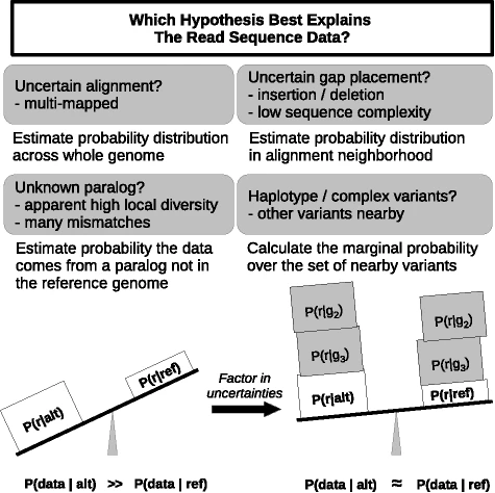
\includegraphics[width=0.6\columnwidth]{body/image/2-1.png}
    \captionsetup{labelfont=bf}
    \renewcommand{\baselinestretch}{1.0}
    \caption[EAGLE model]{EAGLE use generative probabilistic model handle probabilistically.}
    \label{f2-1}
\end{figure}
 

Overall, the more uncertain the data the more uncertain the explanation, Thus, in principle the likelihood computed by EAGLE can be used rank the reliability of putative variants.
\section{Reference Bias}
Sequencing data analysis often begins with aligning reads to a reference genome, but this sequence only contains reference allele at polymorphic sites. \cite{martiniano2020removing}, it will leads to reference bias (Figure \ref{f2-2}): for reads that contain alternate alleles, tend to misalignment or incorrect alignments \cite{chen2021reference}, and due to reference bias, at heterozygous site, the reads containing the reference allele constitute the majority of the reads, these situations can cause false negative or false positive variant calls. \cite{gunther2019presence}

\begin{figure}[H]
    \centering
    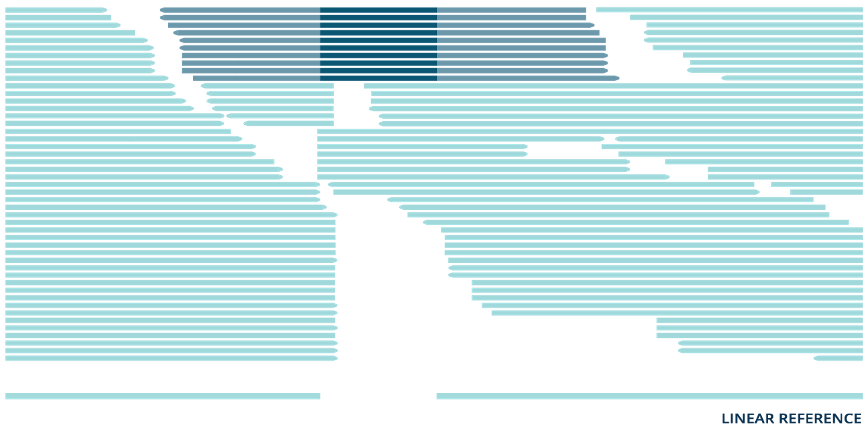
\includegraphics[width=1\columnwidth]{body/image/2-2.png}
    \captionsetup{labelfont=bf}
    \renewcommand{\baselinestretch}{1.0}
    \vspace{-1cm}
    \caption[Reference bias]{Reference bias. Only a small portion of the read containing inserts (dark blue) are mapped to the correct positions during the alignment to the reference genome.}
    \label{f2-2}
\end{figure}
 

There have some studies discuss how to mitigated reference bias, such as genome graph aligners \cite{garrison2018variation} \cite{li2020design}, or using high-coverage NGS data, and 
improve the reference genome so that it includes the genomic diversity of the entire population.
In this paper, we modify the reference sequence to include alternate alleles, and try to find some matching reads to support this hypothetical sequence, then add these reads to the calculation of EAGLE to discuss the impact of this method on reducing reference bias and improve the accuracy of assessing variation.



\chapter{Method} \label{ch:3-method}
	\hspace{24pt}
In this chapter, we will introduce the method we added to EAGLE to reduce reference bias; explain in detail how we create our hypothetical sequence based on the variant and how to quickly search through an FM-index to obtain those missing reads, and finally add these reads to the pileup that EAGLE considers.
\section{Overview}
The red area in Figure~\ref{core-workflow} shows our implementation of the core workflow of reducing reference bias on EAGLE, and the whole Figure \ref{core-workflow} is our complete workflow after combining EAGLE. 
We can roughly divide our workflow into the following five parts:

\begin{enumerate}
\item Combine variant information in a VCF file and the reference genome to create a hypothetical sequence which includes individual differences.
\item Build a \textit{read-index}, an FM-index of the read sequences.
\item Use BWA and the read-index to find the reads that match the variant, and then check if they already exists in the pileup.
\item For any reads not found in the pileup, create that read's alignment information mapped against reference sequences 
\item Add read and alignment information to the pileup, to improve the EAGLE calculation.
\end{enumerate}

\begin{figure}[H]
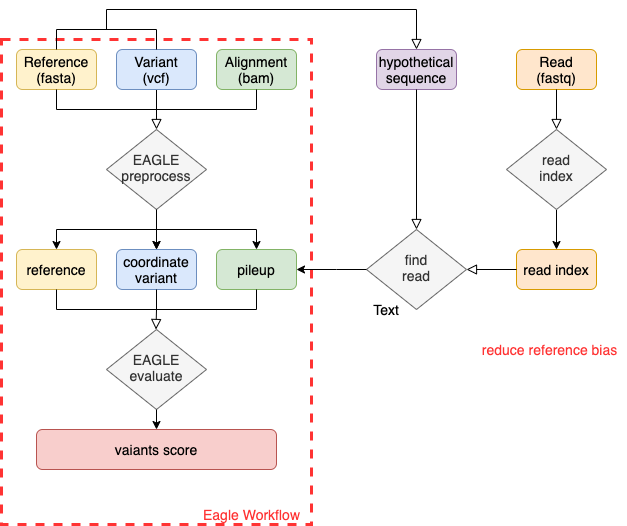
\includegraphics[width=0.8\columnwidth]{body/image/core-workflow.png}
\caption[Core workflow]{The core workflow of EAGLE after adding reference bias reduction.}
\label{core-workflow}
\end{figure}

\section{Hypothetical Sequence}
To reduce the impact of reference bias, the first step we need to construct a hypothetical sequence. Before constructing hypothetical sequence we need variation data and a reference genome. VCF is the standard file format for storing variation data, used by most variant callers (Figure \ref{VCF-format}). FASTA is reference genome format (Figure \ref{FASTA-format}), and it is a text-based format for representing either nucleotide sequences or peptide sequences.

\begin{figure}[H]
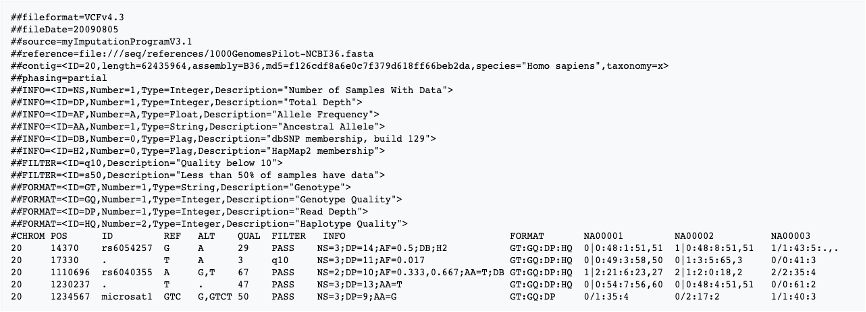
\includegraphics[width=1\columnwidth]{body/image/VCF-format.png}
\caption[VCF format]{Example for VCF format.}
\label{VCF-format}
\end{figure}

\begin{figure}[H]
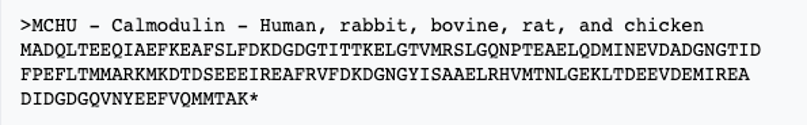
\includegraphics[width=1\columnwidth]{body/image/FASTA-format.png}
\caption[FASTA format]{Example for FASTA format.}
\label{FASTA-format}
\end{figure}

One of the reasons for reference bias is that the reference genome cannot contain individual differences. And our hypothetical sequence is a sequence that combines reference genome and variant. Because we simulate the occurrence of mutation of the reference sequence by combining variant, it includes individual differences. Thus, bases on the information of each variant in the VCF file, including variant position (POS), chromosome name (CHROM), sequence before mutation (REF), and sequence after mutation (ALT), we generate a hypothetical sequence. 

For each hypothetical sequence, according to the variant position, we replace sequence before mutation (REF) to sequence after mutation (ALT). At the same time we will extract the reference genome part front and back in this region, and the length will be the length of a read. The length of this area is long enough to get all the reads we are interested in and also includes individual differences. Figure~\ref{construct-hyposeq} illustrates in detail how we generate a hypothetical sequence based on different types of variants.

We hope to find a read that matches our hypothetical sequence in the FASTQ file to achieve the effect of reducing the reference bias.

\begin{figure}[H]
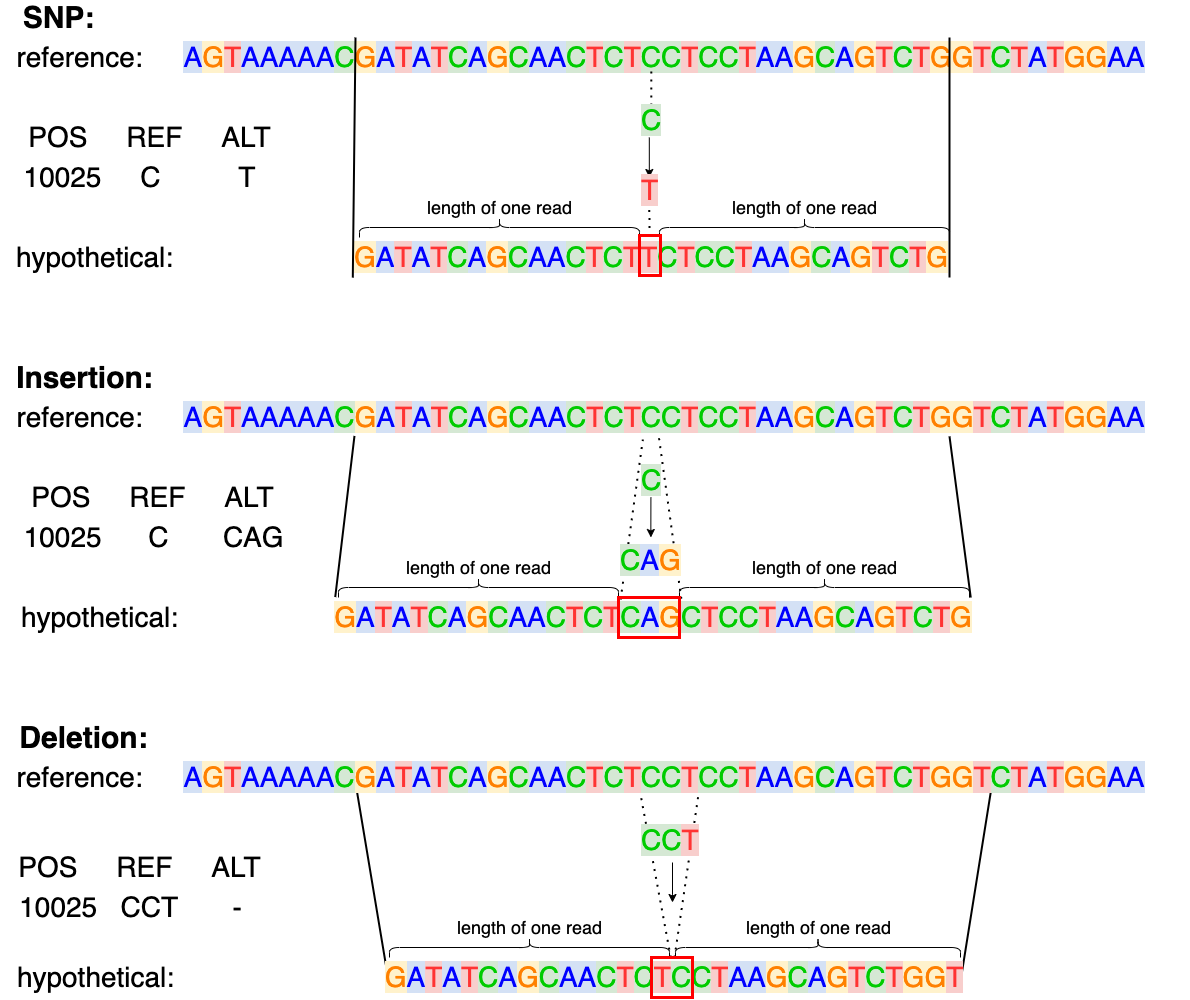
\includegraphics[width=1\columnwidth]{body/image/construct-hyposeq.png}
\caption[construct hypothetical sequence]{Three different cases to construct hypothetical sequence.}
\label{construct-hyposeq}
\end{figure}

\section{Read-index}

Following is an important step for us to find the read that matches our hypothetical sequence. However, if we simply search for matching reads in the FASTQ file, it will cost us a lot of time. 

First we describe general practice: the supposed genome sequence is the reference genome, and we need to map reads on this, just like alignment. Therefore we need to construct index for each hypothetical sequence and then query all the read in FASTQ file. As we mentioned above, we need $O(n\log n)$  ($n$ is reference sequence length) to construct BWT index, and querying will cost $O(\ell)$ ($\ell$ is read length) for each read.

In general situation, the time spent to build an index and perform queries is:
%%
\begin{equation*}
O(n \log n) + O(\ell)
\end{equation*}

It is indeed a very efficient method for standard applications. It only needs to query once for each read, because all reads only need to be aligned to one reference genome sequence. But in our situation, our hypothetical genome sequence is not constant. For each variant we will establish a hypothetical sequence, so if we follow the traditional method, we need to search all the reads every time. Our speed will be very slow.

What would the situation will be if we construct index for read and used our hypothetical sequence to query?
%%
\begin{enumerate}
\itemsep=0em
\item We just need to build index once a time.
\item For each hypothetical sequence, our query will be very fast.
\end{enumerate}


\noindent Let's take an example and some assumptions:


In general situations, we need to create an index for each hypothetical sequence and do a complete read search. It will take time:
\begin{equation*}
\mathlarger{\sum_{h\in H}} \Big\{ \text{build index on } h + \sum_{r\in R}\text{query}~r~\text{on that index} \Big\}
\end{equation*}
where $H$ denotes the set of hypothetical sequences (one for each variant) and $R$ denotes the set of reads.

\begin{flushleft}
Since the hypothetical sequences are very short compared to the combined length of all reads, the time spent on index building can be ignored.  Query time is linear in the total length of the queries so the time needed is approximately:
\begin{equation*}
\mathlarger{\sum_{h\in H}} \Big\{ \sum_{r\in R}\text{query}~r~\text{on index} \Big\} = |H| \times \ell\,|R|
\end{equation*}
Where $|H|$ denotes the number of hypothetical sequences, $\ell$ the read length, and $|R|$ the number of reads.

On the other hand, when building an index on the reads instead of the hypothetical sequences

And through our way of creating a read index, the time would be:
\begin{equation*}
\text{build index on } R + \sum_{h\in H} \text{query}~h \; \approx \; \ell\,|R|\; \log( \ell|R| ) + 2 \ell\,|H|
\end{equation*}
Which is much faster.
\end{flushleft}

According to the above results, we decided to index our reads to generate and read-index, which helps us quickly find reads matching and sequence. Before indexing, we need to remove some information in read file to convert FASTQ format to FASTA format. This is very simple as we describe in Table \ref{tab:FastaToFastq}, then we can directly call BWA index function to construct read-index.

\begin{table}[ht]
\caption{The difference between FASTQ and FASTA format}
\setlength{\tabcolsep}{1mm}{
\begin{tabular}{|c|l|l|l|}
\hline
\rowcolor{gray} 
\multicolumn{2}{|l|}{\cellcolor{gray} }  & \multicolumn{1}{c|}{\cellcolor{gray} {\color{white} \textbf{Fasta}}} & 
\multicolumn{1}{c|}{\cellcolor{gray} {\color{white} \textbf{Fastq}}}\\
\hline
\rowcolor{lightgray}\cellcolor{gray}& 
Line 1 & description of sequence & @sequence id   \\ 
\cline{2-4} 
\cellcolor{gray}&
Line 2  & sequence & sequence \\
\cline{2-4} 
\rowcolor{lightgray}\cellcolor{gray}&
Line 3  & & +\\ 
\cline{2-4} 
\multirow{-4}{*}{\cellcolor{gray}{\color{white} \textbf{format}}} &
Line 4  & & quality value\\ 
\hline
\rowcolor{lightgray}
\multicolumn{2}{|c|}
{\cellcolor{gray}} & $>$NT\_113878.1 chrom1 & @SEQ\_ID \\
\rowcolor{lightgray}
\multicolumn{2}{|c|}
{\cellcolor{gray}} & \footnotesize{\texttt{GATAGTAGTTGCAGCAGGCTAGCTA}} & \footnotesize{\texttt{GATAGTAGTTGCAGCAGGCTAGCTA}} \\
\rowcolor{lightgray}
\multicolumn{2}{|c|}
{\cellcolor{gray}} & & +    \\
\rowcolor{gray}
\multicolumn{2}{|c|}
{\multirow{-4}{*}{\color{white} \textbf{example}}} &\cellcolor{lightgray} &\cellcolor{lightgray}\footnotesize{\verb|???DB+=2C>??E;>C>??EEEFF;|} \\ \hline
\end{tabular}
}
\label{tab:FastaToFastq}
\end{table}

\section{Find Similar Reads}
In previous section, we have introduced how BWA-MEM work, and in this section, we will introduce how we use BWA and the read-index to find the reads that matched hypothetical sequences and filter them.

Like EAGLE, BWA is an open-source software implemented in C.  Fortunately, we can directly use the functions of BWA-MEM and modify part of the code according to EAGLE needs to make it meet our read-index search requirements. Basically, we will use seed alignment based on super maximal exact matching to search for our hypothetical sequence.

The following will describe the changes we made meet to our needs. First of all, for the original BWA-MEM, a read will have only one best matching position, and the others will be marked as secondary (or no primary) (Figure \ref{secondary-alignment}), but for our purposes we simply want to collect all reasonable matches (Figure \ref{primary-alignment}).

\begin{figure}[H]
\vspace{1em}
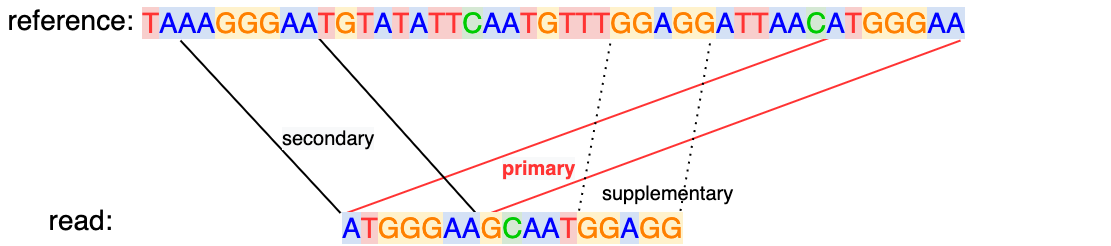
\includegraphics[width=1\columnwidth]{body/image/secondary-alignment.png}
\caption[secondary alignment]{BWA secondary alignment, supplementary alignment.}
\label{secondary-alignment}
\end{figure}

\begin{figure}[H]
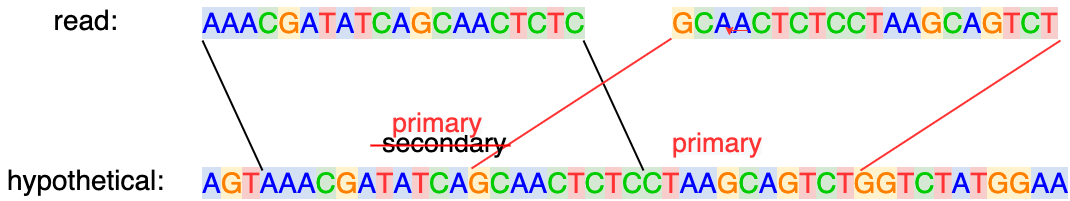
\includegraphics[width=1\columnwidth]{body/image/primary-alignment.png}
\caption[primary alignment]{The read index is used to find reads matching a hypothetical genome sequence.  BWA marks some matches as primary, etc., but we treat them all the same.}
\label{primary-alignment}
\end{figure}

Then we use BWA-MEM to search for our hypothetical sequence using seed alignment based on super maximal exact match, after this, we will get two sets of index as Figure \ref{read-index} shows, one set represents the start and end positions of the region on the hypothetical sequence, and the other set represents the index of the corresponding read region on the read-index. 

\begin{figure}[H]
\vspace{1em}
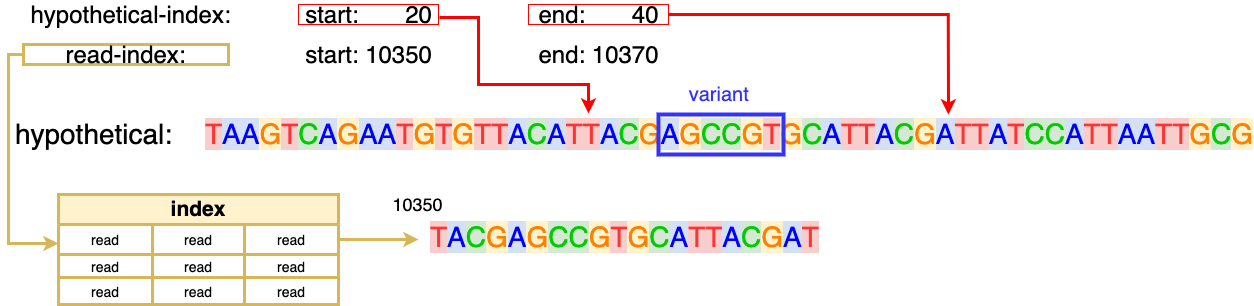
\includegraphics[width=1\columnwidth]{body/image/read-index.png}
\caption[read-index]{how to find matching read through read-index.}
\label{read-index}
\end{figure}

Through the index of hypothetical sequence, we can check whether it contains the variant, if not, we will filter it, as Figure \ref{filter-reads} shows.  At the end of this step, we can obtain a set of reads meeting our requirements, and then add them to the pileup.

\begin{figure}[H]
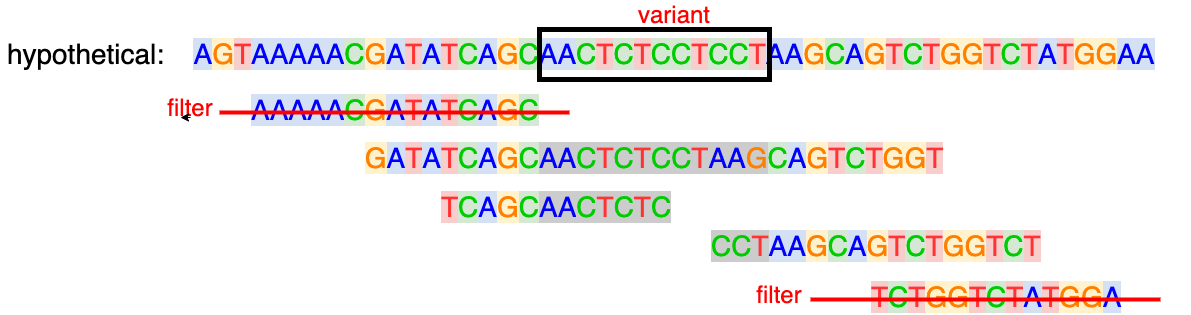
\includegraphics[width=1\columnwidth]{body/image/filter-reads.png}
\caption[Filter reads]{Filter reads that don't overlap the variant.}
\label{filter-reads}
\end{figure}

\section{Integrating new reads into the pileup}
In the last step, we need to compare all the read sets obtained in the previous step with the reads in the pileup. What is the pileup?
We start with a standard read mapping result stored in BAM file format.  We can observe that reads is mapped to a position in the reference genome. Many reads may align to the same region, and this ``pile'' of reads is called the pileup. Our final goal is to find reads that overlap with the same variant position but do not exist in the BAM file, (Figure \ref{exp-pileup} shows the pileup reads which overlap on a variant position.)

\begin{figure}[H]
\vspace*{1em}
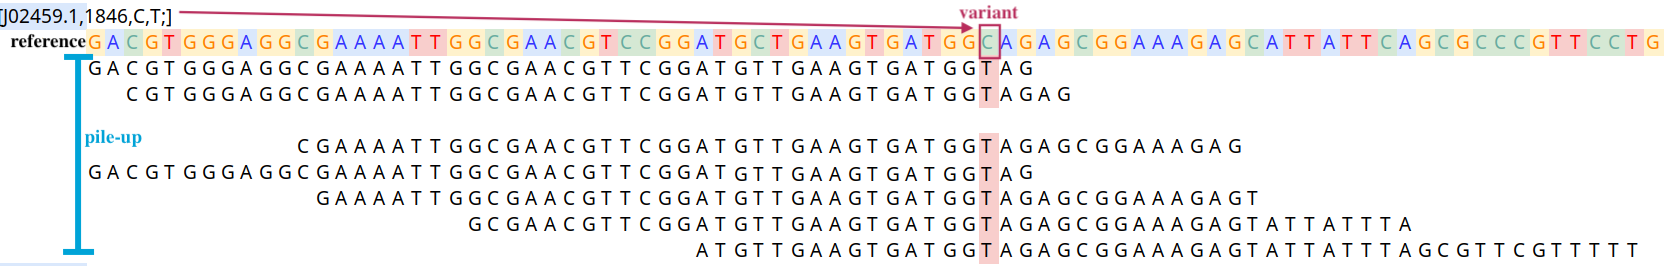
\includegraphics[width=1\columnwidth]{body/image/exp-pileup.png}
\caption[pileup]{pileup at the variant position.}
\label{exp-pileup}
\end{figure}

We can get the pileup from a BAM file quickly through the utility library \texttt{HTSlib}, and then compare the read set with these pileup reads, if the read does not exist in the pileup, it means that we have got the results we want.  The next step for our work is to convert this read, and use the two sets of index obtained in the previous step to generate some essential information that will be needed in our eagle calculation, including SAM flag and CIGAR string, SAM flag is represents the mapping status of this read and the CIGAR string encodes the detailed alignment of the read. We will explain how we get CIGAR string through two sets of indexes.

If we get the SAM flag and CIGAR directly through our two sets of indexes, what we get is the alignment information of hypothetical sequence mapping to read, like previous Figure \ref{read-index} shows, but what EAGLE needs is the alignment information of read mapping to reference sequence. So we need do some processing on the match positions.

First of all, from the position of matches to in read-index, we can directly obtain matching reads.  The other match position is relative to the start and end of our hypothetical sequence --- a length $2\ell$ sequence containing a candidate variant in the middle.  We need to convert positions in this sequence into positions in the reference genome to help us add the read to the pileup in such as way that EAGLE can consider it when evaluating that variant.

\noindent
This problem can be divided into 4 cases(Figure \ref{alignment-read}):
%%
\begin{enumerate}
\itemsep=-0.5em
\item the tail of read sequence overlaps with the variant.
\item the front of read sequence overlaps with the variant.
\item the center of read sequence overlaps with the variant.
\item all of read sequence overlaps with the variant.
\end{enumerate}


\begin{figure}[H]
\centering
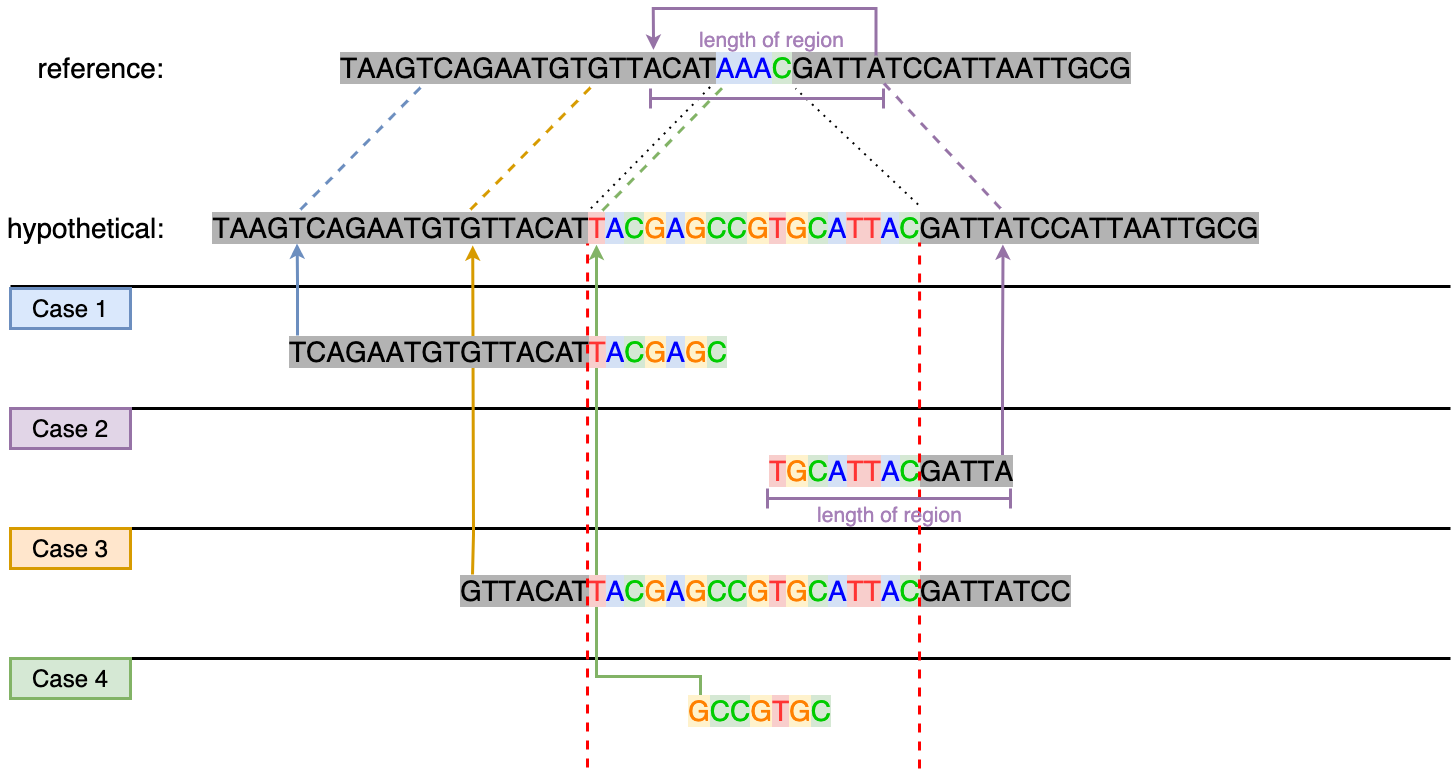
\includegraphics[width=1\columnwidth]{body/image/alignment-read.png}
\caption[alignment read]{Four cases related read to variant.  A read may overlap with part of a variant (left or right side), may completely include a variant, or be included by the variant.}
\label{alignment-read}
\end{figure}


For the first case and third case we can just directly get the reference position, and fourth case we use the position of variant.  In the second case, we need to use the end of the region to push-back the position.

In the last step, we already have read mapping position in the reference genome, so that we can create read alignment information. Most of them are nothing special and will not change as we change the alignment position, except for CIGAR string, we need to convert it from hypothetical sequence's alignment information mapped against read to the read's alignment information mapped against reference sequences (Figure \ref{convert-CIGAR}).  We use a small function we implemented to construct a CIGAR string for these reads.

\begin{figure}[H]
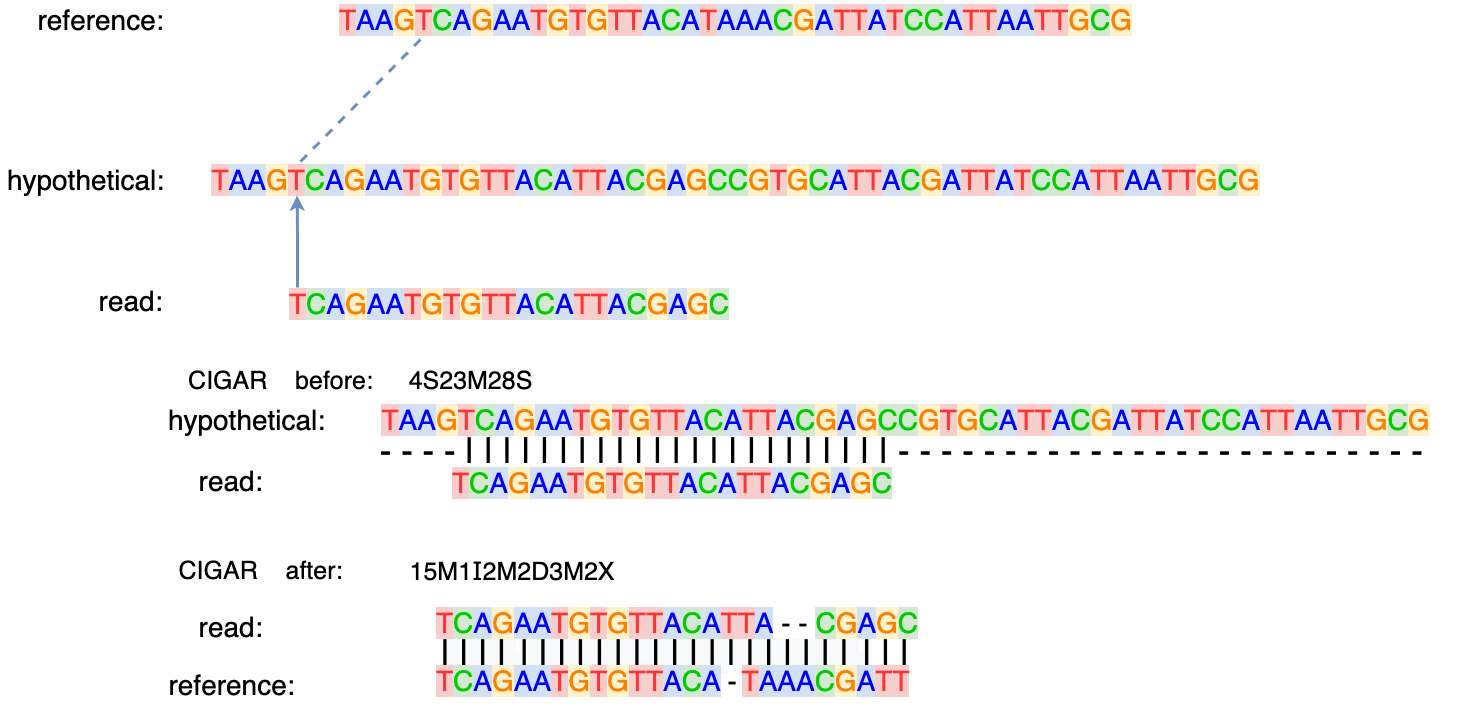
\includegraphics[width=1\columnwidth]{body/image/convert-CIGAR.png}
\caption[CIGAR strings]{How to convert CIGAR strings.}
\label{convert-CIGAR}
\end{figure}

Through these steps we can add read to the pileup for eagle to calculate likelihood.

	
\chapter{Experiment and Results} \label{ch:4-experiment and results}
	\hspace{24pt}
In this section, first we introduce dataset and some tools, then we will explain the steps of our experiment, analyze the experimental results in three different simulation scenarios, and finally discuss results using the VCF file from dbSNP divided it into SNPs and indels.

\section{Dataset}
EAGLE needs three main input files: the reference genome (FASTA), read data (FASTQ), and a variant file (VCF). 

First, the reference genome sequencing data we used is Genome Reference Consortium Human Build 37 patch release 13 (GRCh37.p13) version from NCBI website.  It includes autosomal chromosomes 1 to 22, X and Y chromosome of primary assembly and some extra sequences.

Second, the read sequencing data is real sequencing data from NA12878 which is a cell line of an individual female from a CEPH pedigree that is Utah residents with Northern and Western European ancestry, using an exome sequencing dataset (Garvan HG001) by sequencer HiSeq2500 from Genome-In-A-Bottle (GIAB).

Third, we will use VCF files from the Single Nucleotide Polymorphism Database (dbSNP). dbSNP is a public domain archive for a wide collection of simple genetic polymorphisms. The polymorphism set includes single bases nucleotide substitutions (also called single nucleotide polymorphisms or SNPs), and small-scale base deletions or insertions (indels).

Finally, we will also use a simulated VCF file, the variant file is generated by our simulation, we provide more details below.

\section{Simulation workflow}
In order to carefully evaluate the effect of our modifications to EAGLE and verify whether our method can reduce the influence of reference bias, we use simulation methods to conduct experiments.  We modify the GRCh37 reference genome sequence to simulate the occurrence of differences between a reference genome and an individual genome (Figure~\ref{simulate_variants}), and record the result of our modification to generate a VCF file.  We refer to variants simulated in this way as ``planted variants'' and the resulting modified reference as the ``doctored reference''.  An advantage of this approach is real read data can be used.  A disadvantage is that only homozygous variants can be simulated.

\begin{figure}[ht]
\vspace{1em}
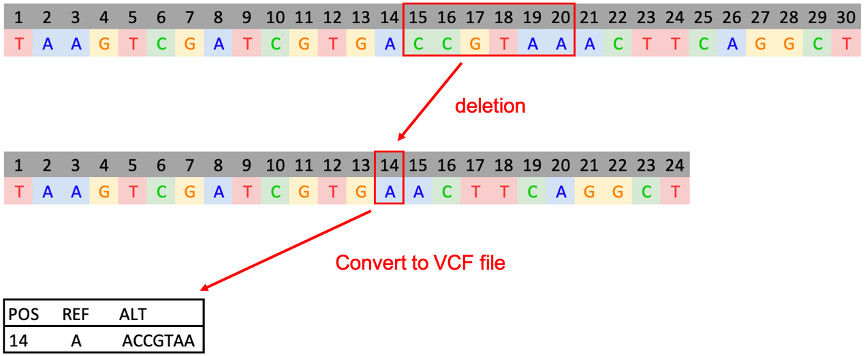
\includegraphics[width=1\columnwidth]{body/image/simulate_variants.png}
\caption[Simulate variants]{Simulate variants.}
\label{simulate_variants}
\end{figure}

Then we will use BWA, following the traditional approach, and do the read mapping alignment again, to obtained a doctored reference pile-up.  Use the re-alignment step to simulate the occurrence of reference bias, because we modified the reference, when re-aligning, the pileup at the original position will have some reads affected by the change we made to the reference, and these affected reads will be misaligned or perhaps mapped elsewhere. After generating the files needed by EAGLE, we can start our experiment.  The entire experiment process is outlined in Figure~\ref{simulation_workflow}.

\begin{figure}[ht]
\vspace{1em}
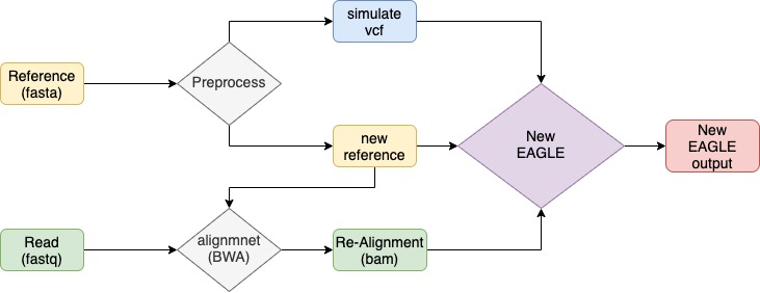
\includegraphics[width=1\columnwidth]{body/image/simulation_workflow.png}
\caption[Simulation workflow]{Simulation workflow.}
\label{simulation_workflow}
\end{figure}

In order to analyze the affect of read depth on our results, we used SAMtools to check the original reference pile-up read depth, and divide genome positions into three categories of pileup read depth: 5--20x, 20--40x and \textgreater40x (Table~\ref{tab:simulate-amount}).

\vspace{0.5cm}
\begin{table}[ht]
\center
\caption[total simulate indels amount]{total simulate indels amount}
\vspace{-0.5cm}
\begin{tabular}{|l|c|c|c|}
\hline
\rowcolor{lightgray}
\textbf{Pile-up Read Depth}&    \textbf{5x -- 20x} &    \textbf{20x -- 40x} &    \textbf{$>$ 40x}\\
\hline
\cellcolor{lightgray}\textbf{Indel length} &   1 -- 50&     1 -- 50&     1 -- 50\\
\hline
\cellcolor{lightgray}\textbf{Amount} &   20 for each&    20 for each&     20 for each\\
\hline
\cellcolor{lightgray}\textbf{Total variants} &   1000&     1000&     1000\\
\hline
\end{tabular}
\label{tab:simulate-amount}
\end{table}


For each read depth category, and each length $l$ from 1 to 50, we randomly selected 20 positions and deleted a string of $l$ base pairs from the standard reference genome to obtain a doctored reference genome.  We do this to simulate insertion variants, as the read data (which is real and presumably matches the standard reference genome in most positions) should contain the sequences we deleted from the reference.  While examining the affect of indel length on our results we will discuss the results after re-alignment in two situations, one is that after re-alignment to the doctored reference, BWA still aligns some reads to the planted variant position, and the other is that after re-alignment, no read can be aligned to that position.

In the first case, the original EAGLE is still able to evaluate the variants, so the focus of our discussion will be the changes in EAGLE evaluation after the introduction of our method. For the second case, we will focus on the new results calculated by EAGLE.

\begin{samepage}
\noindent
Our evaluation is based on the log odds ratio output of EAGLE of each variant $v$:
%%
\begin{equation*}
\log \frac{\text{P}[\text{Alt} | v]}{\text{P}[\text{Ref} | v]}
\end{equation*}
\end{samepage}


\section{Case 1: Low read depth}
The first two rows of Table \ref{tab:low-variants} show how often the EAGLE likelihood ratio changes after adding any new reads from our read index into consideration.
We can see that in the case of low read depth, since only a small number of reads are mappable at all (even against the original reference sequence), once there is a reference bias (simulated by mapping against the doctored reference), EAGLE's evaluation can easily be severely affected.  As expected, you can also see that the longer the length of indels, the more serious the impact.
\vspace{0.5cm}
\begin{table}[ht]
\center
\caption[low read depth variants]{low read depth variants}
\vspace{-0.5cm}
\begin{tabular}{|l|l|l|l|l|l|l|l|l|l|l|r|}
\hline
\textbf{Indel Length} & 
\multicolumn{2}{c|}{\textbf{1--10}}  & \multicolumn{2}{c|}{\textbf{11--20}}  & \multicolumn{2}{c|}{\textbf{21--30}}  &
\multicolumn{2}{c|}{\textbf{31--40}}  & \multicolumn{2}{c|}{\textbf{41--50}}   & 
\textbf{Total}\\\hline
\rowcolor{lightgray}
\textbf{Unchanged}  & 
47 & 42\%       &
38 & 41.8\%     &
30 & 29.1\%    &
10 & 19.2\%     &
0 & 0\%          &
125\\ \hline
\textbf{Changed} & 
65 & 58\%       &
53 & 58.2\%     & 
73 & 70.9\%    & 
42 & 80.8\%     &
5 & 100\%        &
238\\ \hline
\rowcolor{lightgray}    
\textbf{New}  & 
\multicolumn{2}{c|}{88}      &
\multicolumn{2}{c|}{109}     &
\multicolumn{2}{c|}{97}      &
\multicolumn{2}{c|}{148}    &
\multicolumn{2}{c|}{195}       & 
637\\ \hline
\end{tabular}
\label{tab:low-variants}
\end{table}

Next, let’s take a look at the changes after adding our read-index based method.  As shown in table~\ref{tab:low-variants-change}, EAGLE predicts that the position does not contain variants when only using the doctored reference pile-up; but in most cases (19 out of 23), when we find some reads matching the variants, we can help EAGLE judge whether the position contains variants. 

\begin{table}[ht]
\center
\caption{Number of planted variants missed at low read depth}
\begin{tabular}{|l|c|c|c|c|c|r|}
\hline
\diagbox[dir=NW,width=12em]{$\frac{\mathbf{P}[\text{Alt}]}{\mathbf{P}[\text{REF}]} < 1$}{\textbf{Indel length}} &
\textbf{1--10} & \textbf{11--20} & \textbf{21--30} & \textbf{31--40} & \textbf{41--50} & \textbf{Total}\\
\hline
\rowcolor{lightgray}
\textbf{Before} &  7&     2&     3&    4&   3&   19 \\
\hline
\textbf{After} &   2&     1&     0&    1&   0&    4 \\
\hline
\end{tabular}
\label{tab:low-variants-change}
\end{table}

We checked the cases that changed after we found the read, and we found that most of the examples were as we predicted, and we were able to find reads that were misaligned due to reference bias. Figure~\ref{low_new_ALTread} is one of the cases.

\begin{figure}[H]
\centering
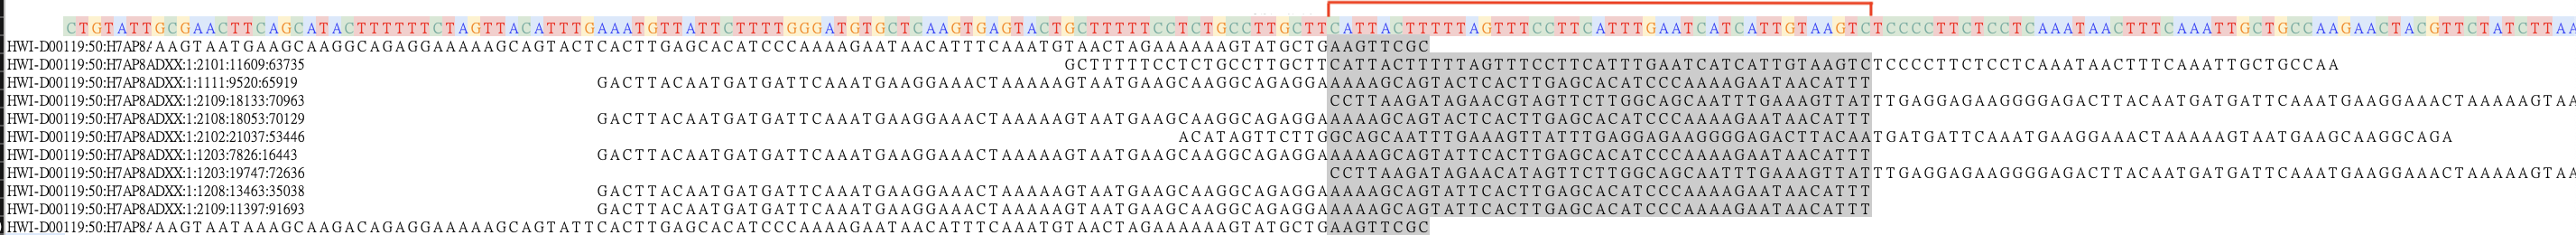
\includegraphics[width=1\columnwidth]{body/image/low_new_ALTread.png}
\caption[New reads in a region with low pile-up read depth]{Example of new reads supporting a variant in a region with low pile-up read depth.}
\label{low_new_ALTread}
\end{figure}

Similarly, especially in repetitive genome regions, there are some new reads which are also similar to the reference sequence (Figure \ref{low_new_REFread}).

\vspace{1cm}
\begin{figure}[H]
    \centering
    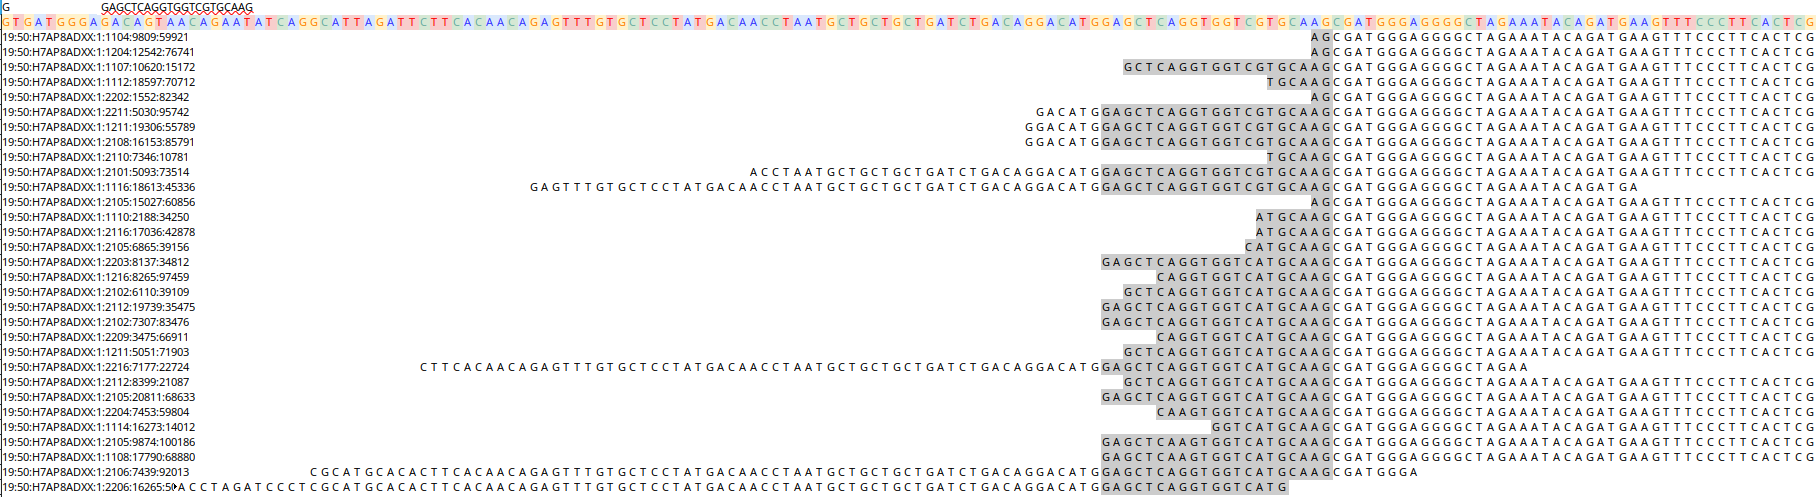
\includegraphics[width=1\columnwidth]{body/image/low_new_REFread.png}
    \captionsetup{labelfont=bf}
    \renewcommand{\baselinestretch}{1.0}
    \vspace{-1cm}
    \caption[New reads are similar to the reference with low pile-up read depth]{Example where new reads found are also similar to the reference sequence with low pile-up read depth.  Note the repetitive nature of the surrounding genome sequence.}
    \label{low_new_REFread}
\end{figure}

Next, we can look at the comparison of EAGLE log odds ratio.
\begin{equation*}
\text{log odds ratio change} = \text{log odds(after)} - \text{log odds(before)}
\end{equation*}
to represent the effect of our new method on EAGLE candidate variant evaluation.

\vspace{1cm}
\begin{figure}[H]
    \centering
    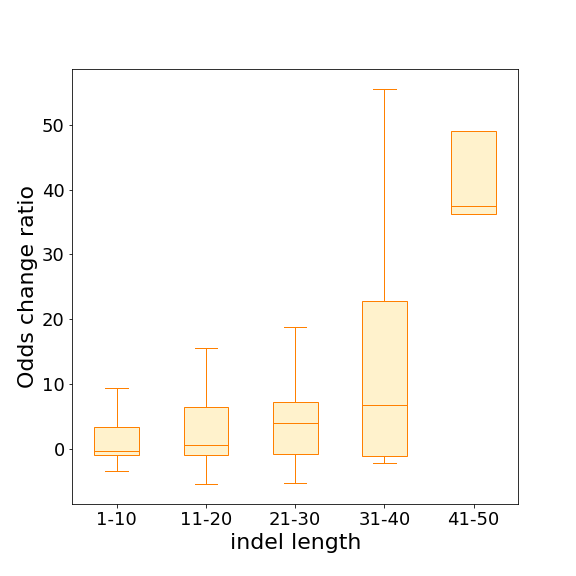
\includegraphics[width=0.6\columnwidth]{body/image/low_odds_change.png}
    \captionsetup{labelfont=bf}
    \renewcommand{\baselinestretch}{1.0}
    \caption[low pile-up read depth odds change ratio]{The vertical axis shows the change in EAGLE log odds ratio of variant to reference for indel variants, grouped by length (horizontal axis).  Change here meaning the difference in the log odds ratio when when using the read index versus only using the pile-up.  Plotted for variants from low pile-up read depth regions.}
    \label{low_odds_change}
\end{figure}

In the case of low pile-up read depth, first of all, we can observe that after we add reads, the confidence value of most of the variants increases because we find more reads that contain the variant sequence (Figure \ref{low_odds_change}), and regardless of the length of the indel, their distribution of logs odds ratio change is mostly above zero.
This may mean that even in the case of low pile-up read depth, our method is very helpful for most mutation points, especially for indels with a length of 40 or more, where the increase is particularly obvious.

Finally, we look at the last row of Table \ref{tab:low-variants-change}, we can see these positions are affected by the reference bias, so that no read can be mapped to these positions to form a pileup. Our method is obviously very helpful. For the remaining variants in the 1,000 variants, we can find those reads that are affected by reference bias and are lost, thereby helping EAGLE evaluate the possibility of these mutations.

\vspace{0.5cm}
\begin{figure}[H]
    \centering
    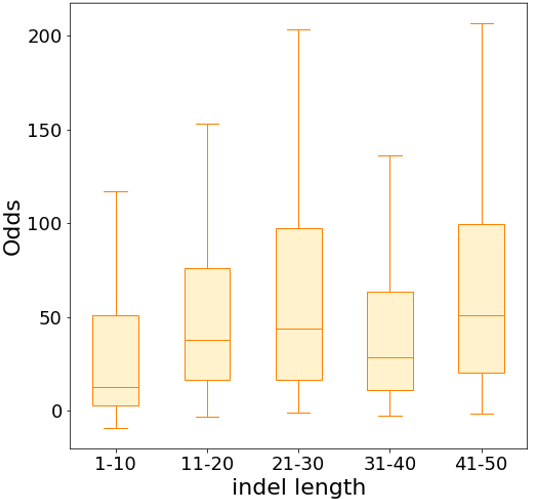
\includegraphics[width=0.6\columnwidth]{body/image/low_new_odds.png}
    \captionsetup{labelfont=bf}
    \renewcommand{\baselinestretch}{1.0}
    \caption[no reads with variants from low pile-up depth odds ratio]{The vertical axis shows the EAGLE log odds ratio of variant to reference for indel variants, grouped by length (horizontal axis).  Plotted for variants occurring in regions with no reads from low pile-up depth.}
    \label{low_new_odds}
\end{figure}

Then see the odds calculated by EAGLE after we find the read (Figure \ref{low_new_odds}), we can see the odds calculated by EAGLE. For most of the variants, EAGLE gives the conclusion the variant occurs at this position, which is also in line with our expected results.


\section{Case 2: Medium pile-up read depth}
\begin{center}
\begin{table}[h]
    \centering
    \caption[medium pile-up read depth variants]{medium pile-up read depth variants}
    \vspace{-0.5cm}
    \begin{tabular}{|l|l|l|l|l|l|l|l|l|l|l|r|}
    \hline
    \textbf{Indel Length} & 
    \multicolumn{2}{c|}{\textbf{1--10}}  & \multicolumn{2}{c|}{\textbf{11--20}}  & \multicolumn{2}{c|}{\textbf{21--30}}  &
    \multicolumn{2}{c|}{\textbf{31--40}}  & \multicolumn{2}{c|}{\textbf{41--50}}   & 
    \textbf{Total}\\\hline
    \rowcolor{lightgray}
    \textbf{Unchanged}  & 
    36 & 28.3\%       &
    21 & 13.4\%     &
    25 & 15.8\%    &
    33 & 20.4\%     &
    22 & 17.1\%          &
    137\\ \hline
    \textbf{Changed} & 
    91 & 71.7\%       &
    136 & 86.6\%     & 
    133 & 84.2\%    & 
    129 & 79.6\%     &
    107 & 82.9\%        &
    596\\ \hline
    \rowcolor{lightgray}    
    \textbf{New}  & 
    \multicolumn{2}{c|}{72}      &
    \multicolumn{2}{c|}{41}     &
    \multicolumn{2}{c|}{42}      &
    \multicolumn{2}{c|}{38}    &
    \multicolumn{2}{c|}{71}       & 
    264\\ \hline
    \end{tabular}
    \label{tab:mid-variants}
\end{table}
\end{center}

First of all, we can see that in this case, Table~\ref{tab:mid-variants}, because of the increase in the original pile-up read depth, the variants which cannot be called due to reference bias are significantly reduced, and the number of reads that we can overlap with the variant position also increased. For the same reason, more misaligned reads are affected by reference bias.

\begin{table}[ht]
    \centering
    \caption[Changes in the number of variants with medium pile-up read depth]{Changes in the number of variants with medium pile-up read depth}
    \vspace{-0.5cm}
    \begin{tabular}{|l|c|c|c|c|c|r|}
    \hline
    \diagbox[dir=NW,width=12em]{$\frac{\mathbf{P}[\text{Alt}]}{\mathbf{P}[\text{REF}]} < 1$}{\textbf{Indel length}} &
    \textbf{1--10} &     \textbf{11--20} &    \textbf{21--30} &    \textbf{31--40} &    \textbf{41--50} &    \textbf{Total}\\
    \hline
    \rowcolor{lightgray}
    \textbf{Before} &   10&     11&     9&    6&   5&    41 \\
    \hline
    \textbf{After} &   1&     1&     0&    1&   0&    3 \\
    \hline
    \end{tabular}
    \label{tab:mid-variants-change}
\end{table}

With the same increase in pile-up read depth, In EAGLE’s initial judgment, the computed likelihood that position does not contain the variant has also increased, because more misalignments have occurred. And just for this reason, the more reads that we can find to help EAGLE. Therefore, we can see that after we find the misaligned reads, the affect on variant evaluation has also increased, nearly 91\% of variants in Table \ref{tab:mid-variants-change} have been changed to the correct situation. Figures~\ref{mid_new_ALTread} and \ref{mid_new_REFread} show some examples.


\begin{figure}[H]
\centering
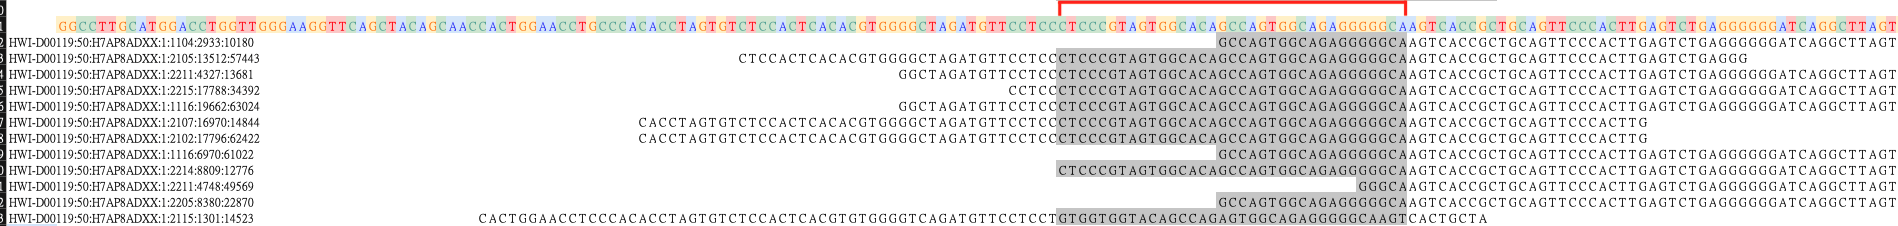
\includegraphics[width=1\columnwidth]{body/image/mid_new_ALTread.png}
\caption[New reads in a region with medium pile-up read depth]{Example of new reads supporting a variant in a region with medium pile-up read depth.}
\label{mid_new_ALTread}
\end{figure}

\begin{figure}[H]
\centering
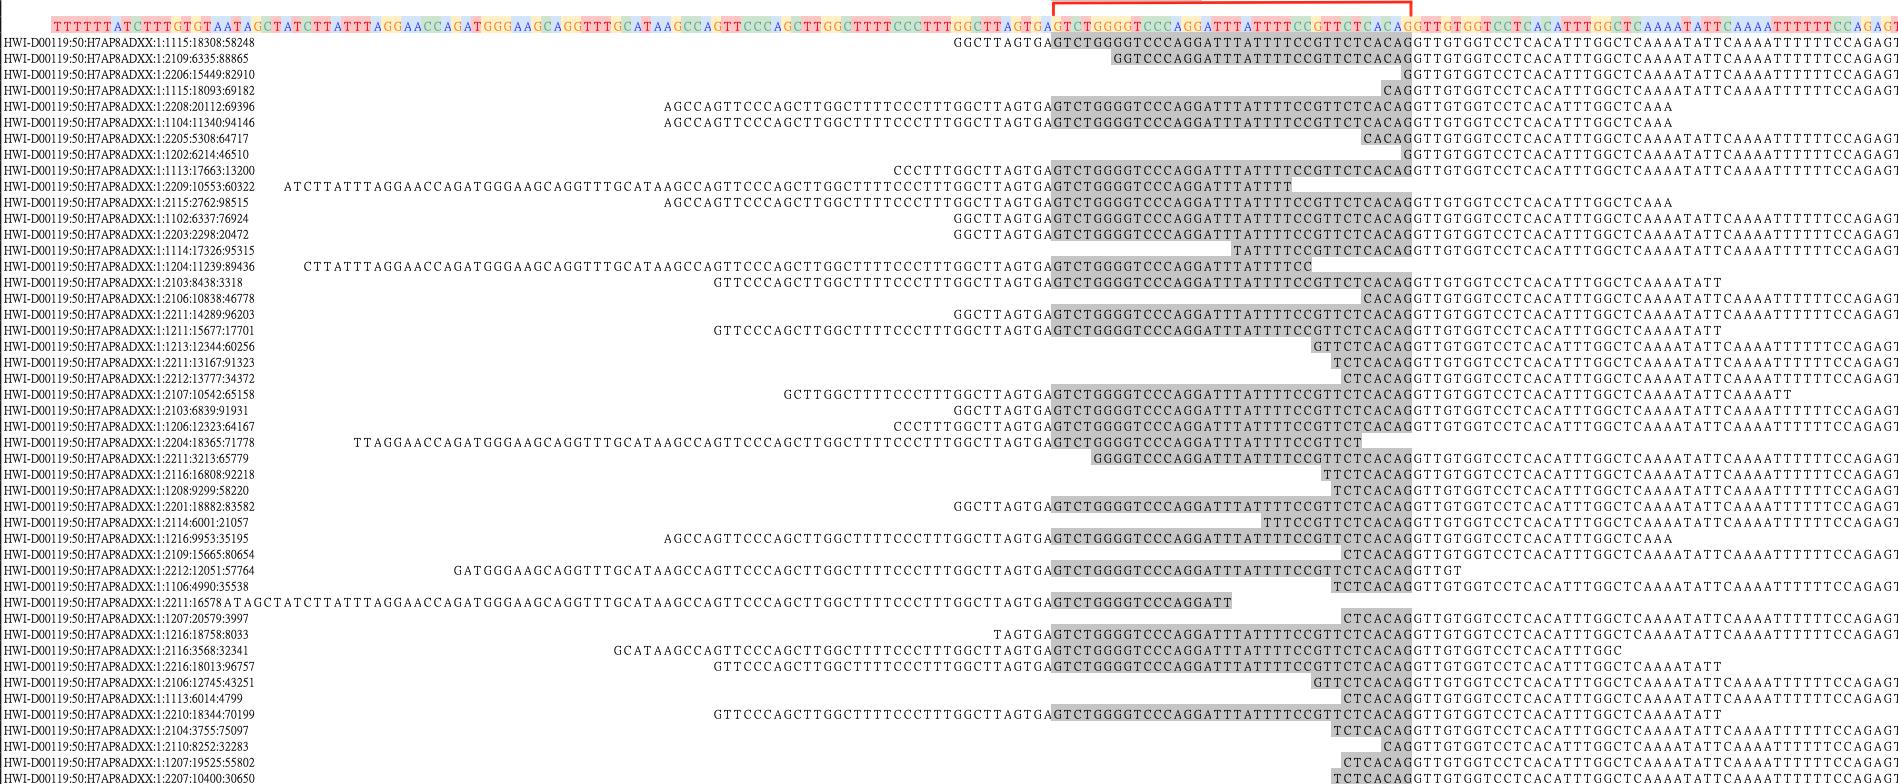
\includegraphics[width=1\columnwidth]{body/image/mid_new_REFread.png}
\caption[New reads are similar to the reference with medium pile-up read depth]{Example where new reads found are also similar to the reference sequence with medium pile-up read depth.  Note the repetitive nature of the surrounding genome sequence.}
\label{mid_new_REFread}
\end{figure}

We can find that in bad cases, although we found reads similar to hypothetical variant sequences, we did not improve the score of EAGLE on variants. In these few examples, we found that their mutated sequences happened to be repeated sequences. Therefore, the similarity between it and the reference sequence is also very high (Figure \ref{mid_pileup_REFread}).

\begin{figure}[H]
\centering
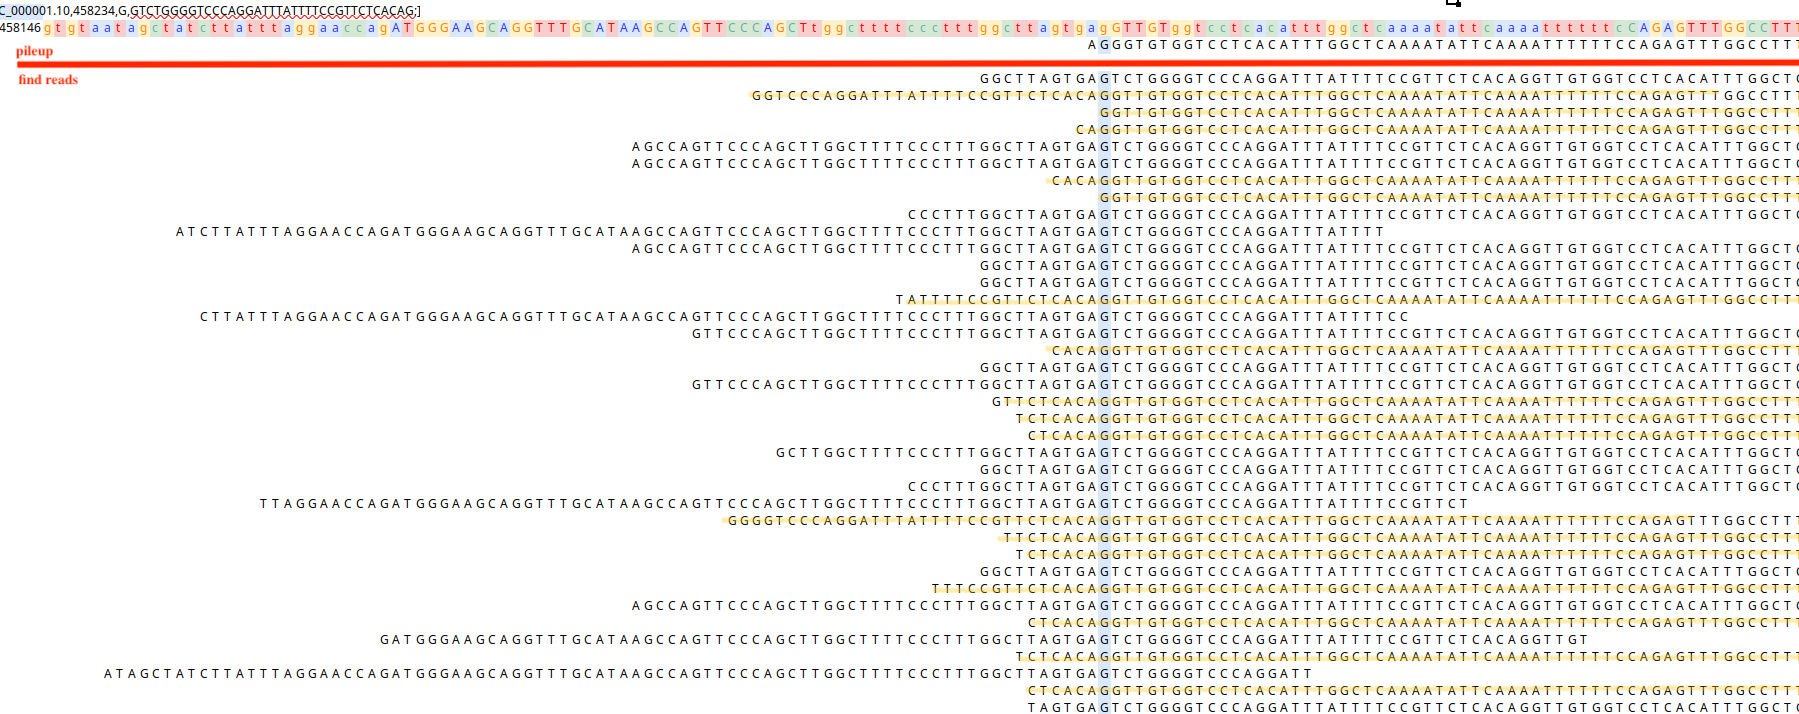
\includegraphics[width=1\columnwidth]{body/image/mid_pileup_REFread.png}
\caption[pileup with Figure \ref{mid_new_REFread}]{pileup with Figure \ref{mid_new_REFread}.}
\label{mid_pileup_REFread}
\end{figure}


\begin{figure}[H]
\centering
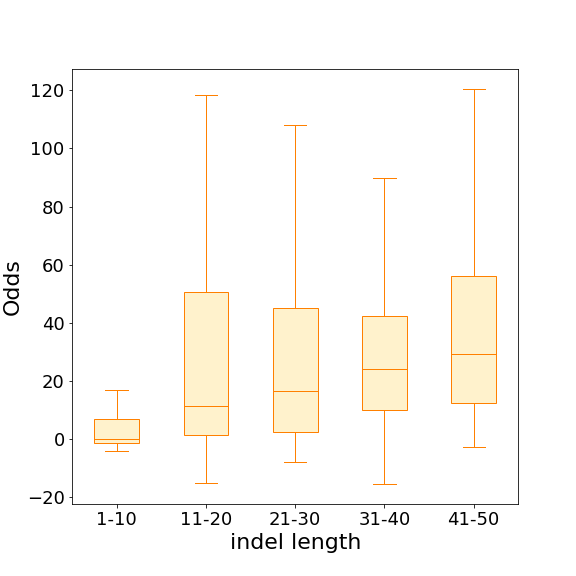
\includegraphics[width=0.6\columnwidth]{body/image/mid_odds_change.png}
\caption[medium pile-up read depth odds change ratio]{The vertical axis shows the change in EAGLE log odds ratio of variant to reference for indel variants, grouped by length (horizontal axis).  Change here meaning the difference in the log odds ratio when when using the read index versus only using the pile-up.  Plotted for variants from medium pile-up read depth regions.}
\label{mid_odds_change}
\end{figure}

Next, we can look at the comparison of EAGLE odds change for medium pile-up read depth (Figure \ref{mid_odds_change}). Basically, the change is similar to the situation of low pile-up read depth. We can also see larger change for longer indels. The difference is that we also have a good performance in the shorter indel. And the average change is better than that of low pile-up read depth. This result is quite reasonable, because we find more reads that match the variant, which can help EAGLE give these mutations greater confidence.
We can also see that indels with a length of 10 or more on our box plot have Q3 greater than 0, which means that most of our reads can help us eliminate the influence of reference bias.

\begin{figure}[H]
\centering
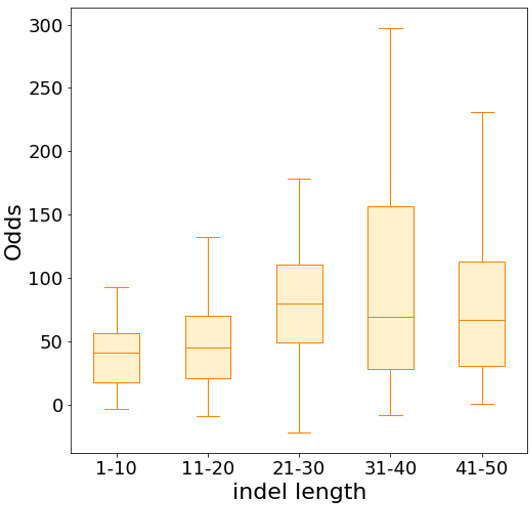
\includegraphics[width=0.6\columnwidth]{body/image/mid_new_odds.png}
\caption[no reads with variants from medium pile-up depth odds ratio]{The vertical axis shows the EAGLE log odds ratio of variant to reference for indel variants, grouped by length (horizontal axis).  Plotted for variants occurring in regions with no reads from medium pile-up depth.}
\label{mid_new_odds}
\end{figure}


Finally, we look at the last row of Table~\ref{tab:mid-variants} we can see that our method still can help some variants that EAGLE cannot calculate because there is no pileup at the position. Figure~\ref{mid_new_odds} shows these variant odds calculated by EAGLE.

In this case, EAGLE can get more correct conclusions, that is, the position does contain variants, because we can find more read support variants. It can be seen that compared to the previous case, regardless of the length of the indel, their Q3 is 0 some distance higher, this result is also as we predicted (for example see Figure~\ref{mid_new_pileup}).


\begin{figure}[H]
\centering
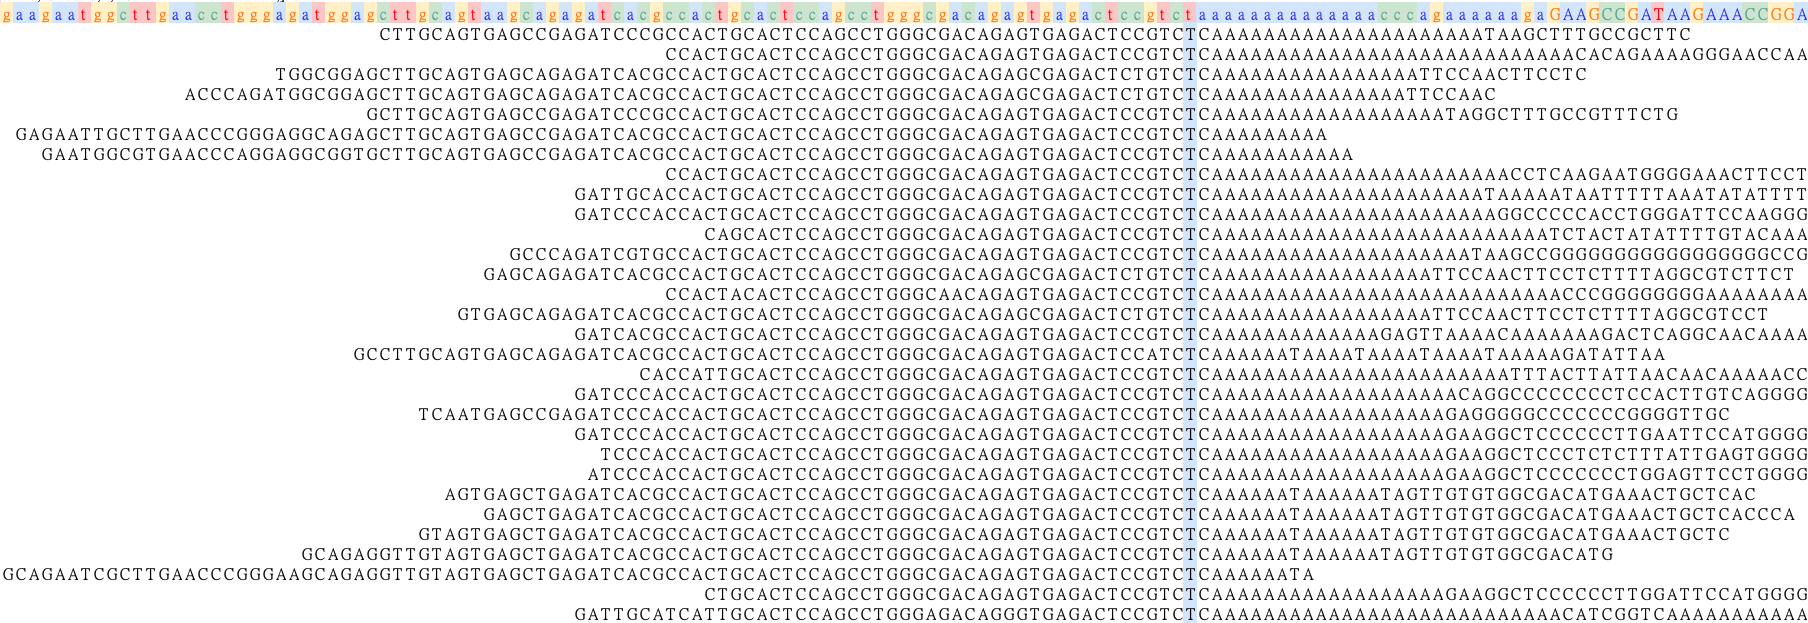
\includegraphics[width=1\columnwidth]{body/image/mid_new_pileup.png}
\caption[find new pileup reads in medium pile-up read depth]{find reads on no pileup position.}
\label{mid_new_pileup}
\end{figure}

\section{Case 3: High pile-up read depth}
\begin{table}[ht]
    \centering
    \caption[high pile-up read depth variants]{high pile-up read depth variants}
    \vspace{-0.5cm}
    \begin{tabular}{|l|l|l|l|l|l|l|l|l|l|l|r|}
    \hline
    \textbf{Indel Length} & 
    \multicolumn{2}{c|}{\textbf{1--10}}  & \multicolumn{2}{c|}{\textbf{11--20}}  & \multicolumn{2}{c|}{\textbf{21--30}}  &
    \multicolumn{2}{c|}{\textbf{31--40}}  & \multicolumn{2}{c|}{\textbf{41--50}}   & 
    \textbf{Total}\\\hline
    \rowcolor{lightgray}
    \textbf{Unchanged}  & 
    44 & 25.9\%       &
    31 & 16.9\%     &
    36 & 19.6\%    &
    4 & 4\%     &
    0 & 0\%          &
    116\\ \hline
    \textbf{Changed} & 
    129 & 74.1\%       &
    152 & 83.1\%     & 
    148 & 80.4\%    & 
    96 & 96\%     &
    80 & 80\%        &
    605\\ \hline
    \rowcolor{lightgray}    
    \textbf{New}  & 
    \multicolumn{2}{c|}{26}      &
    \multicolumn{2}{c|}{17}     &
    \multicolumn{2}{c|}{16}      &
    \multicolumn{2}{c|}{100}    &
    \multicolumn{2}{c|}{120}       & 
    279\\ \hline
    \end{tabular}
    \label{tab:hi-variants}
    %\tabfnt
    {Note: Explain that in the case of high pile-up read depth, after we add read, EAGLE evaluates the number of variants affected.}
\end{table}
\vspace{1cm}

Basically, in this case, we will observe results that are very similar to medium pile-up read depth, that's because there are quite a lot of reads, most positions can still produce pileup (Table \ref{tab:hi-variants}).

\begin{table}[H]
    \centering
    \caption[Changes in the number of variants with high pile-up read depth]{Changes in the number of variants with high pile-up read depth}
    \vspace{-0.5cm}
    \begin{tabular}{|l|c|c|c|c|c|r|}
    \hline
    \diagbox[dir=NW]{\textbf{$P[Alt]/P[REF] < 1$}}{\textbf{Indel length}} &
    \textbf{1--10} &     \textbf{11--20} &    \textbf{21--30} &    \textbf{31--40} &    \textbf{41--50} &    \textbf{Total}\\
    \hline
    \rowcolor{lightgray}
    \textbf{Before} &   6&     6&     2&    35&   36&    85 \\
    \hline
    \textbf{After} &   1&     0&     0&    1&   0&    2 \\
    \hline
    \end{tabular}
    \label{tab:hi-variants-change}
\end{table}

Interestingly, here we observe that the pile-up read depth rate is twice as high as that of the medium pile-up read depth, EAGLE initially judged that the position does not contain variation, but through our method we can complete more corrections than the medium pile-up read depth case. There are nearly 97\% of variants in Table \ref{tab:hi-variants-change} have been changed to the correct situation. (Figure \ref{hi_new_REFread},\ref{hi_pileup_REFread} are some examples)

\begin{figure}[H]
\centering
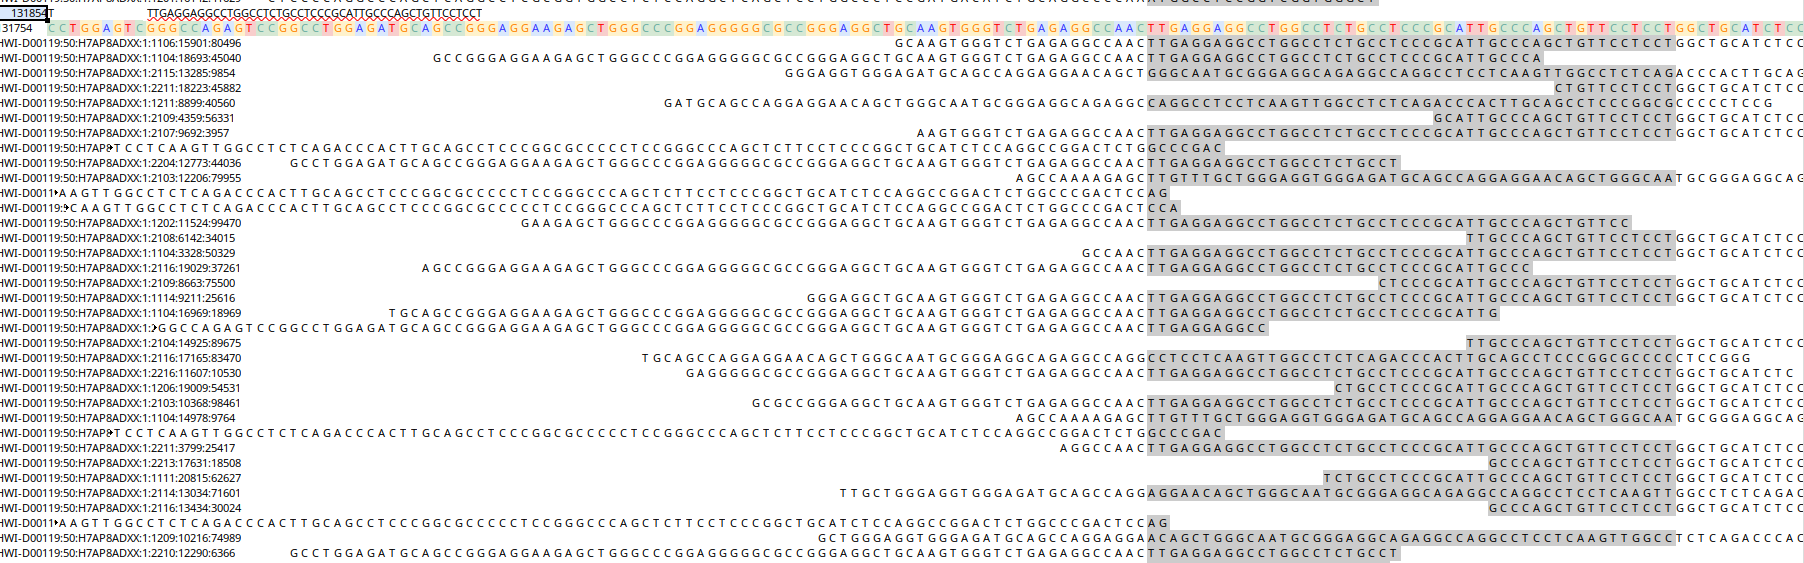
\includegraphics[width=1\columnwidth]{body/image/hi_new_REFread.png}
\caption[New reads in a region with high pile-up read depth]{Example of find large amount new reads supporting a variant in a region with high pile-up read depth.}
\label{hi_new_REFread}
\end{figure}

\begin{figure}[H]
\centering
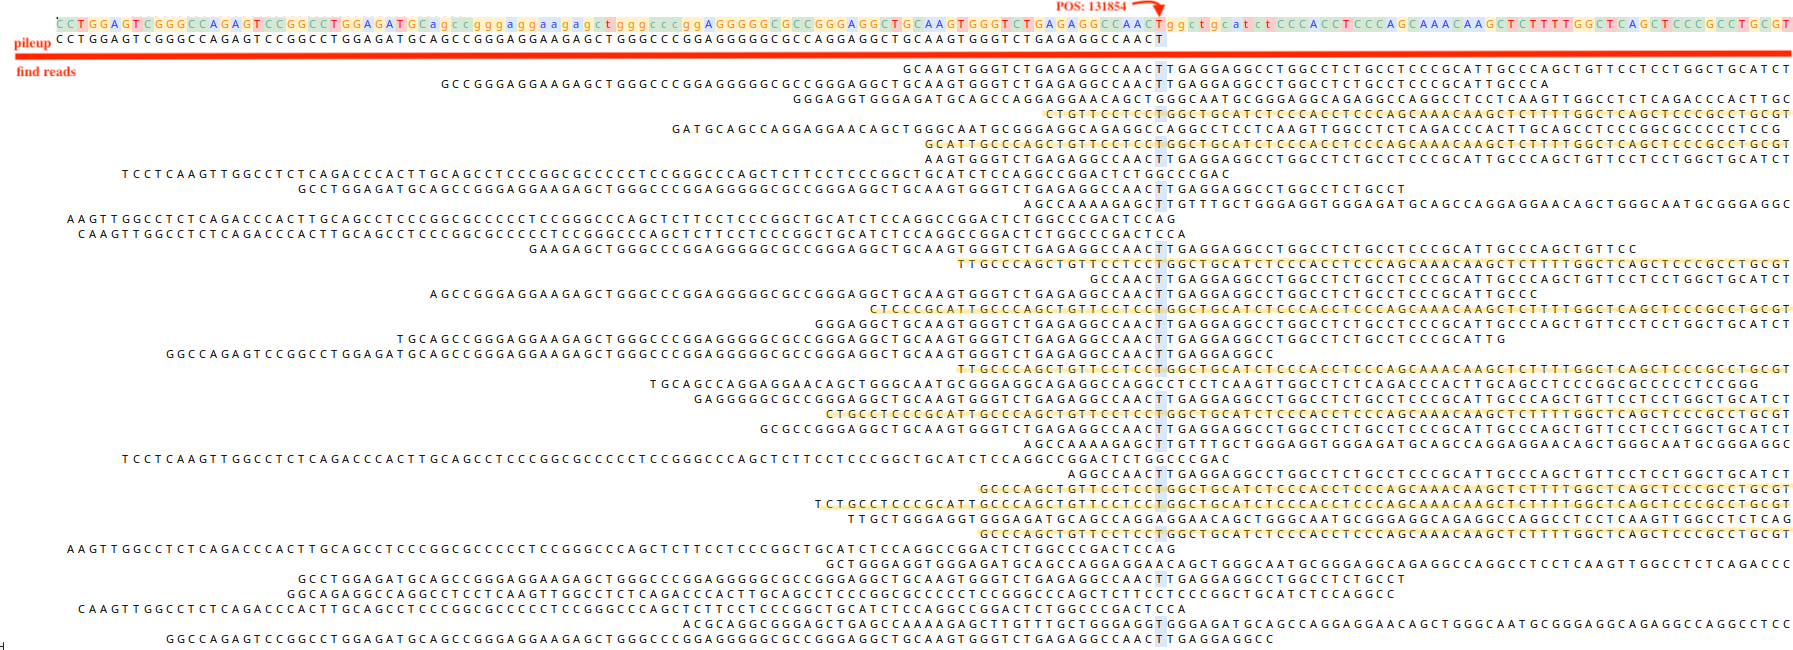
\includegraphics[width=1\columnwidth]{body/image/hi_pileup_REFread.png}
\caption[variant pileup in high pile-up read depth]{Pileup after adding reads.}
\label{hi_pileup_REFread}
\end{figure}

Then, we look at the comparison of EAGLE odds in high pile-up read depth (Figure \ref{hi_odds_change}). It can be seen that compared with the previous example, it is very obvious that the longer the indel, the bigger the increase. However, we found many cases where the length of the mutation is greater than 50. This also shows that the more reads that we can find that would have been lost, the better we can reduce the impact of reference bias.

\begin{figure}[H]
\centering
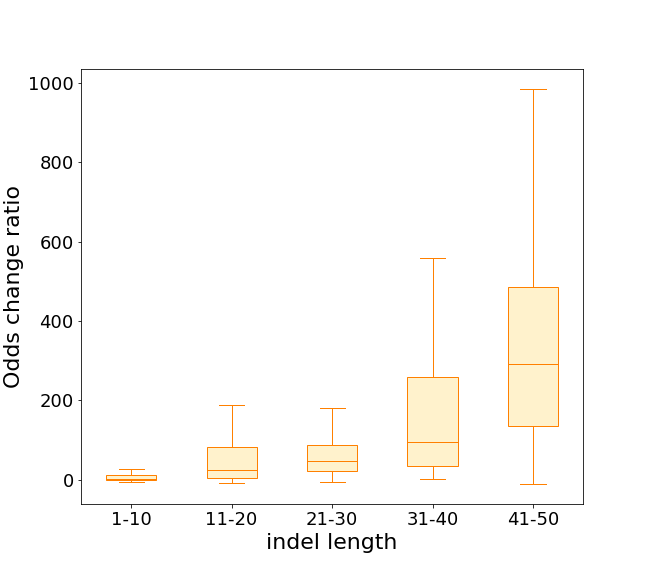
\includegraphics[width=0.6\columnwidth]{body/image/hi_odds_change.png}
\caption[high pile-up read depth odds change ratio]{The vertical axis shows the change in EAGLE log odds ratio of variant to reference for indel variants, grouped by length (horizontal axis).  Change here meaning the difference in the log odds ratio when when using the read index versus only using the pile-up.  Plotted for variants from high pile-up read depth regions.}
\label{hi_odds_change}
\end{figure}

Finally, we look at the last row of Table\ref{tab:hi-variants}, we can see the same result as the previous case medium pile-up read depth. Figure\ref{hi_odds_change} shows these variant odds calculated by EAGLE.

\begin{figure}[H]
\centering
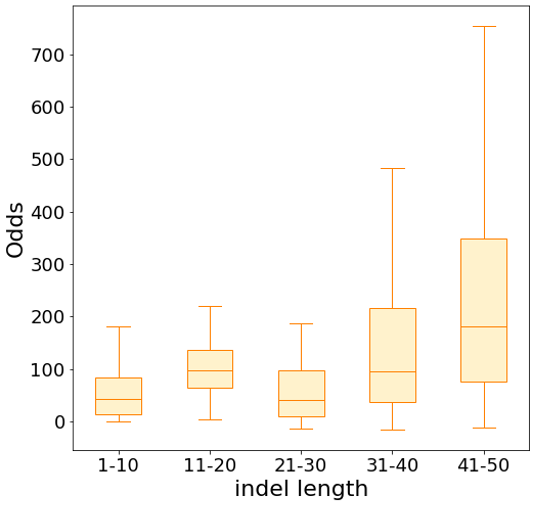
\includegraphics[width=0.6\columnwidth]{body/image/hi_new_odds.png}
\caption[no reads with variants from high pile-up depth odds ratio]{The vertical axis shows the EAGLE log odds ratio of variant to reference for indel variants, grouped by length (horizontal axis).  Plotted for variants occurring in regions with no reads from high pile-up depth.}
\label{hi_new_odds}
\end{figure}


\section{SNPs in dbSNP dataset}

There are 15,936,832 SNP variants form the dpSNP dataset, we random select 100,000 variants from the dataset, and the amount of matching pileup of the querying SNP variants are 50488. After joining our method, there are 22995 variants that have been changed as a result, we have looked at a few cases (Figure \ref{snp_new_ALTread},\ref{snp_pileup_ALTread},\ref{snp_new_REFread},\ref{snp_pileup_REFread}), we find many sequences that include the variants.


\begin{figure}[H]
\centering
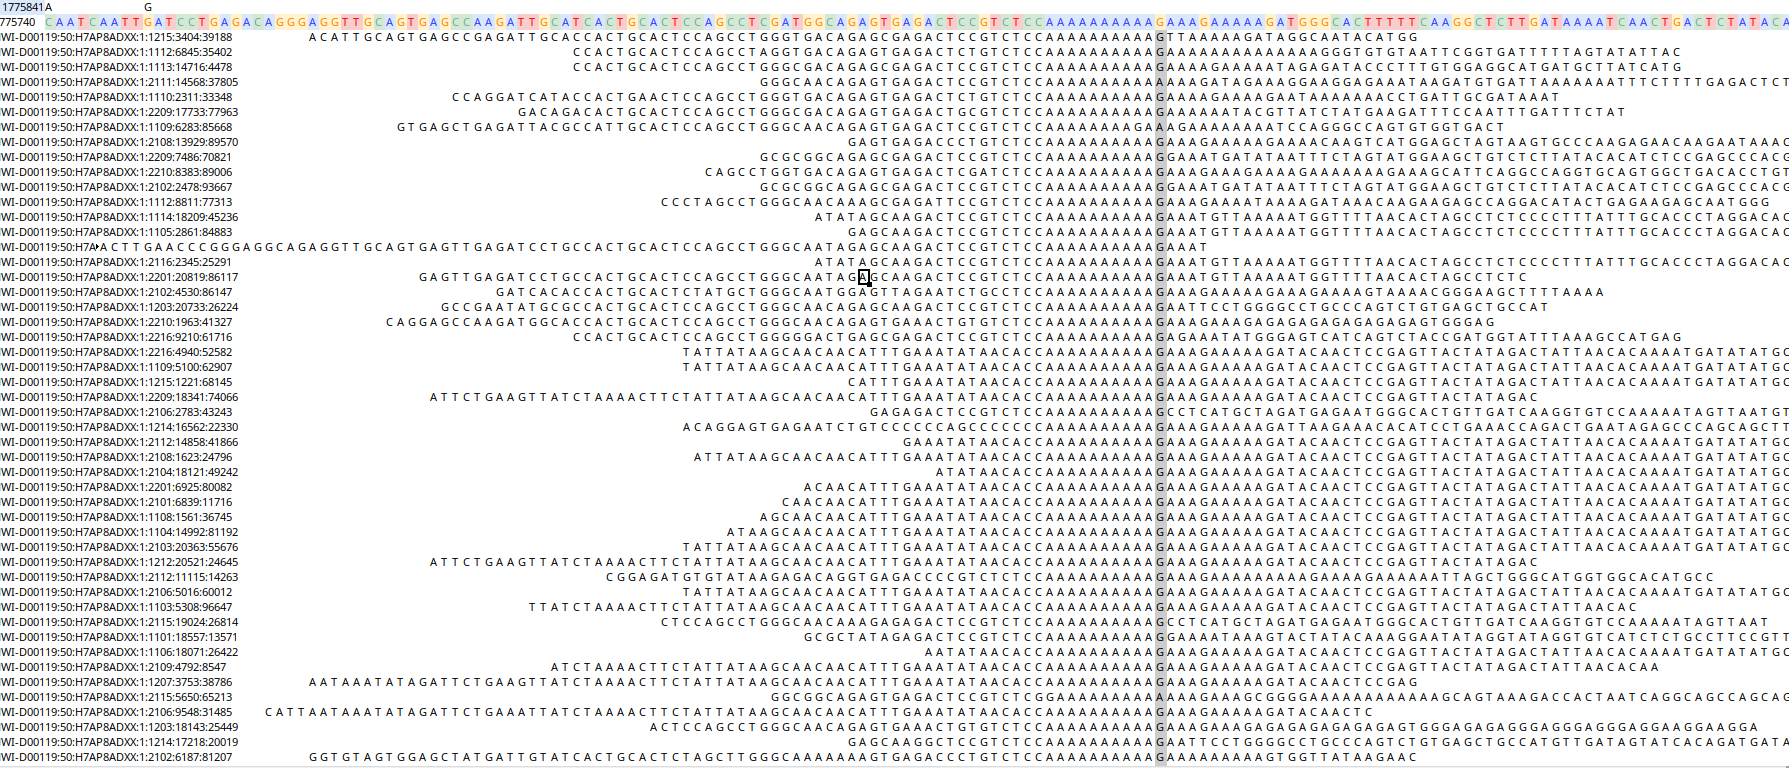
\includegraphics[width=1\columnwidth]{body/image/snp_new_ALTread.png}
\caption[SNP match reads]{ found match reads with hypothetical sequence in SNP.}
\label{snp_new_ALTread}
\end{figure}

\begin{figure}[H]
\centering
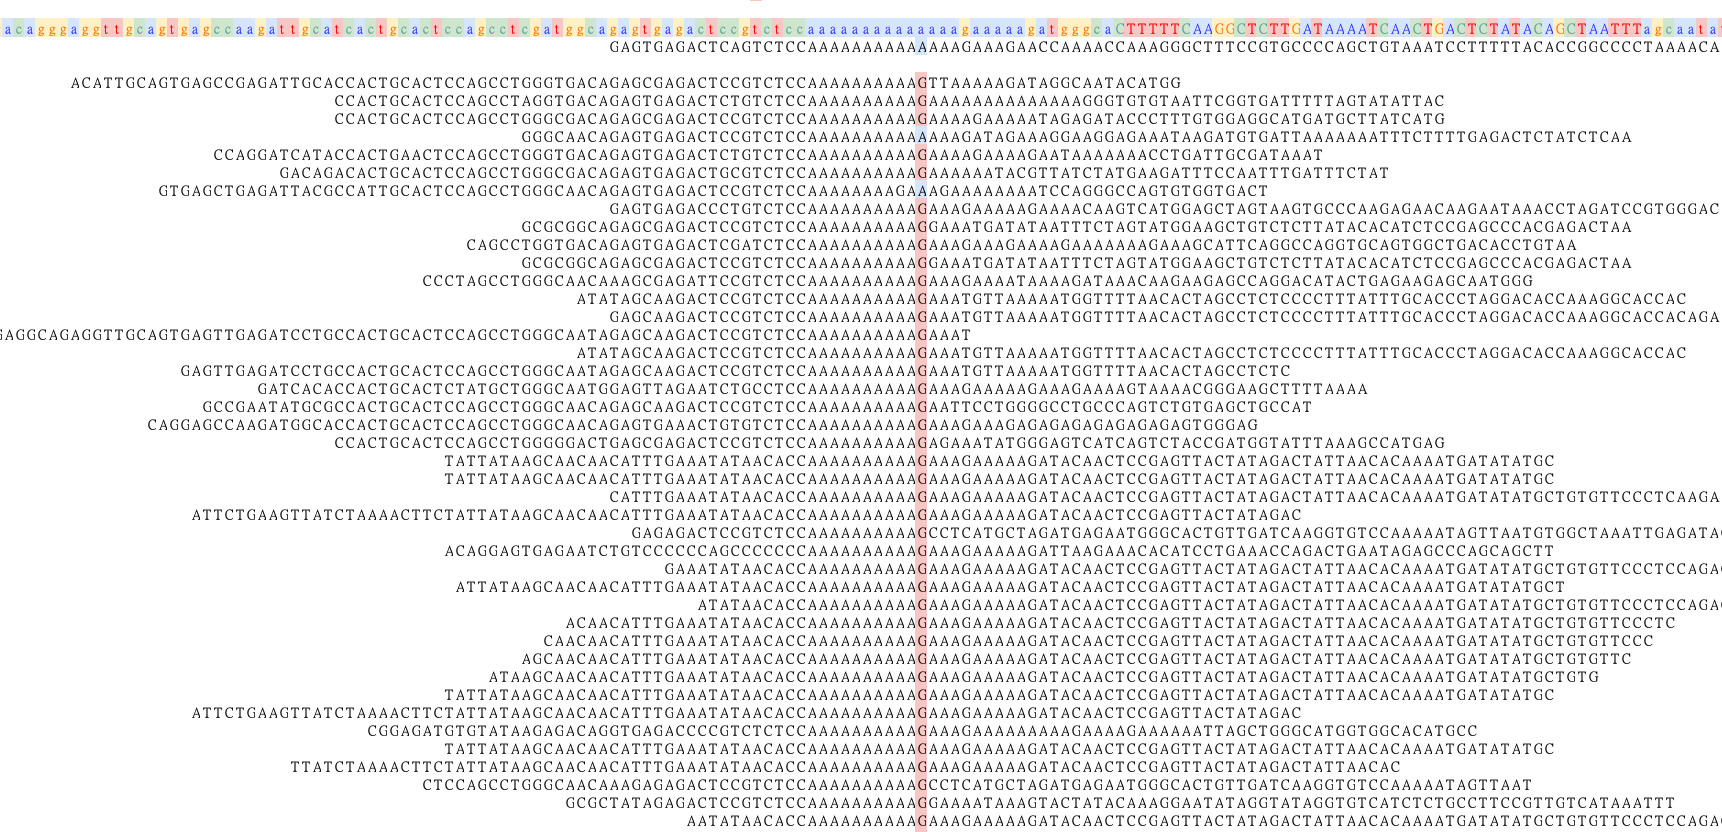
\includegraphics[width=1\columnwidth]{body/image/snp_pileup_ALTread.png}
\caption[Figure 4.17 pileup]{ The pileup corresponding to the Figure \ref{snp_new_ALTread} variants.}
\label{snp_pileup_ALTread}
\end{figure}

\begin{figure}[H]
\centering
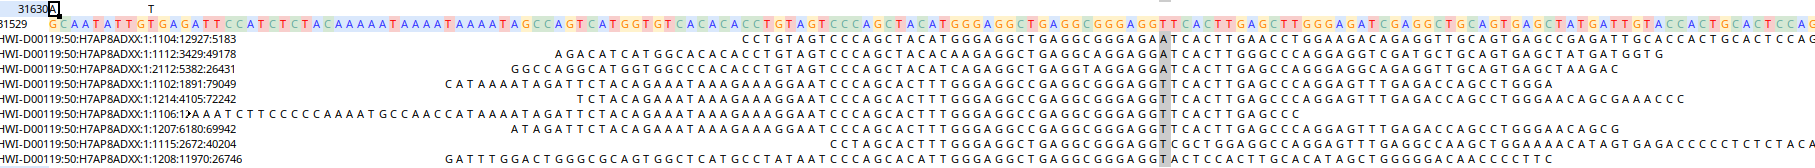
\includegraphics[width=1\columnwidth]{body/image/snp_new_REFread.png}
\caption[SNP worse match reads]{ found match reads but more similar to reference sequence in SNP.}
\label{snp_new_REFread}
\end{figure}

\begin{figure}[H]
\centering
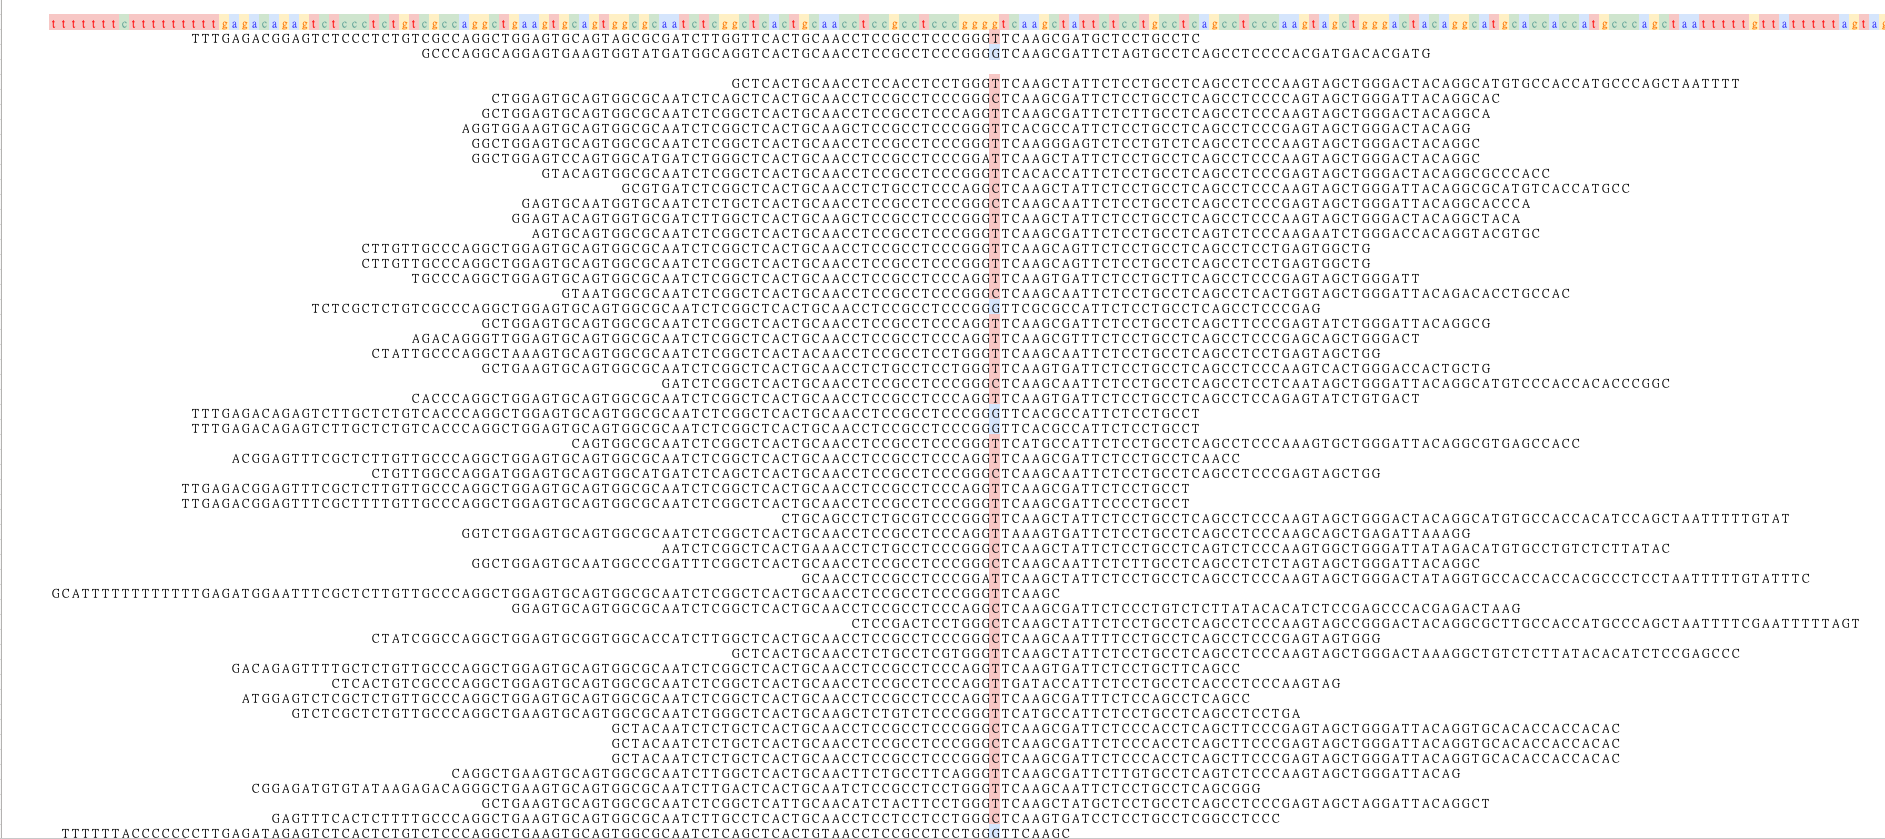
\includegraphics[width=1\columnwidth]{body/image/snp_pileup_REFread.png}
\caption[SNP worse match reads pileup]{The pileup corresponding to the Figure \ref{snp_new_REFread} variants.}
\label{snp_pileup_REFread}
\end{figure}

And we can find that the read we found gives EAGLE more basis for judgment, but the magnitude of the change is not very obvious in the SNPs (Figure \ref{snp_odds_change}), and most of them are less than 0. We speculate that the single-base nucleotide substitutions will not have a great impact on the alignment results.

\begin{figure}[H]
\centering
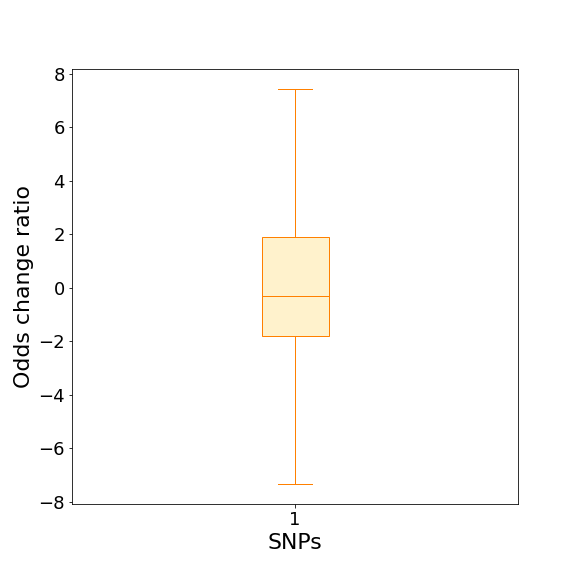
\includegraphics[width=0.6\columnwidth]{body/image/snp_odds_change.png}
\caption[SNPs odds change ratio]{SNPs odds change ratio.}
\label{snp_odds_change}
\end{figure}

\section{INDELs in dbSNP dataset}

There are 1,759,193 INDEL variants form the dpSNP dataset, we random select 10,000 variants from the dataset, and the amount of matching pileup of the querying INDEL variants are 5093. After using our new method, there are 2482 variants that have been changed as a result.  We have looked at a few cases  (Figure \ref{indel_new_ALTread},\ref{indel_pileup_ALTread},\ref{indel_new_REFread},\ref{indel_pileup_REFread}).

\begin{figure}[H]
\centering
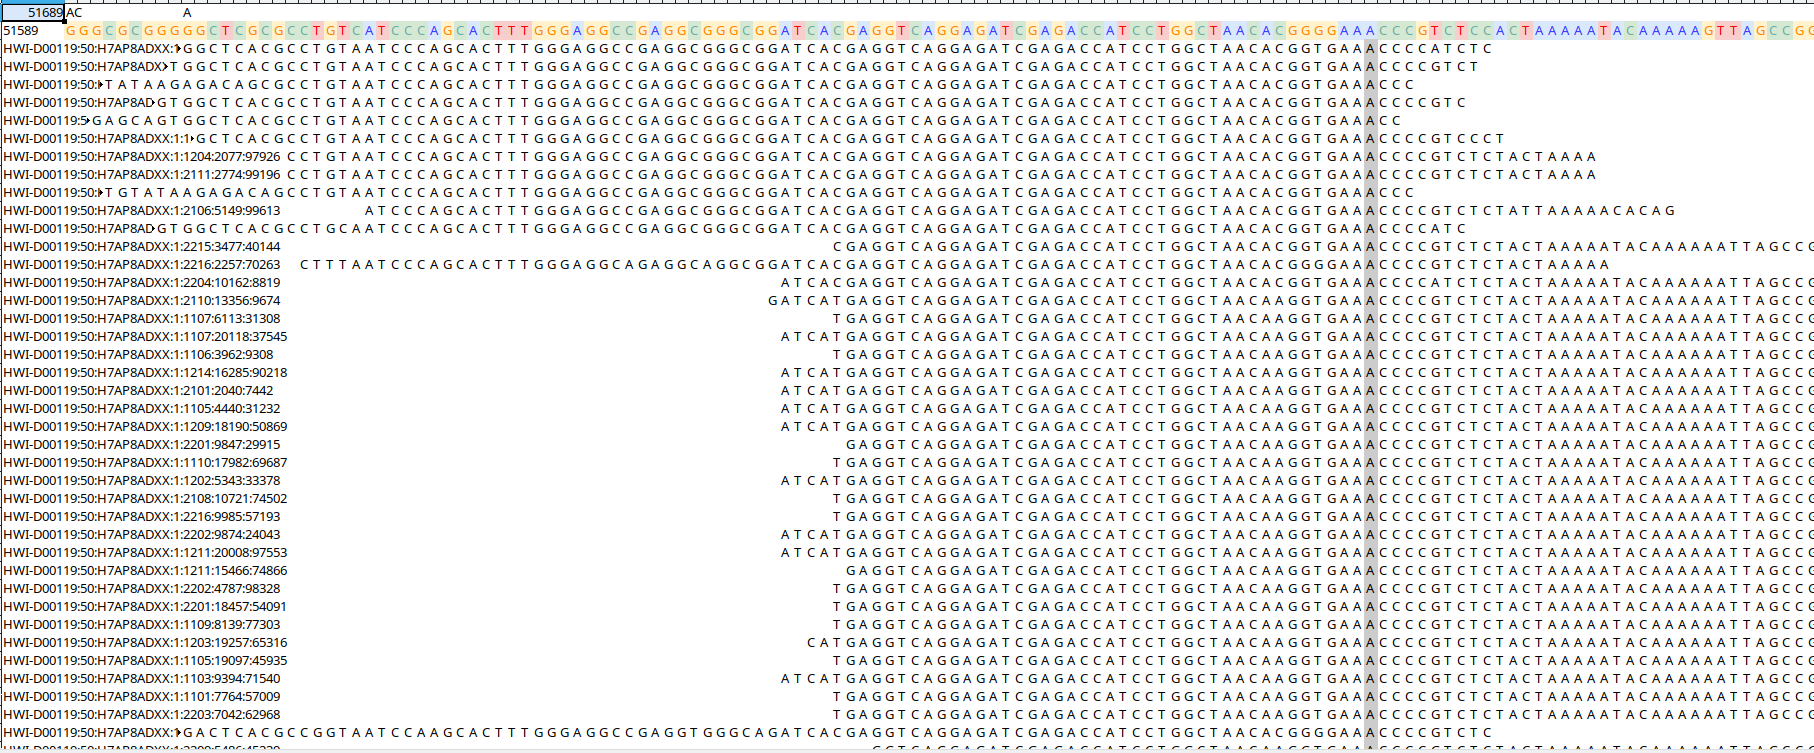
\includegraphics[width=1\columnwidth]{body/image/indel_new_ALTread.png}
\caption[INDEL match reads]{Matching reads with hypothetical sequence in INDEL}
\label{indel_new_ALTread}
\end{figure}

\begin{figure}[H]
\centering
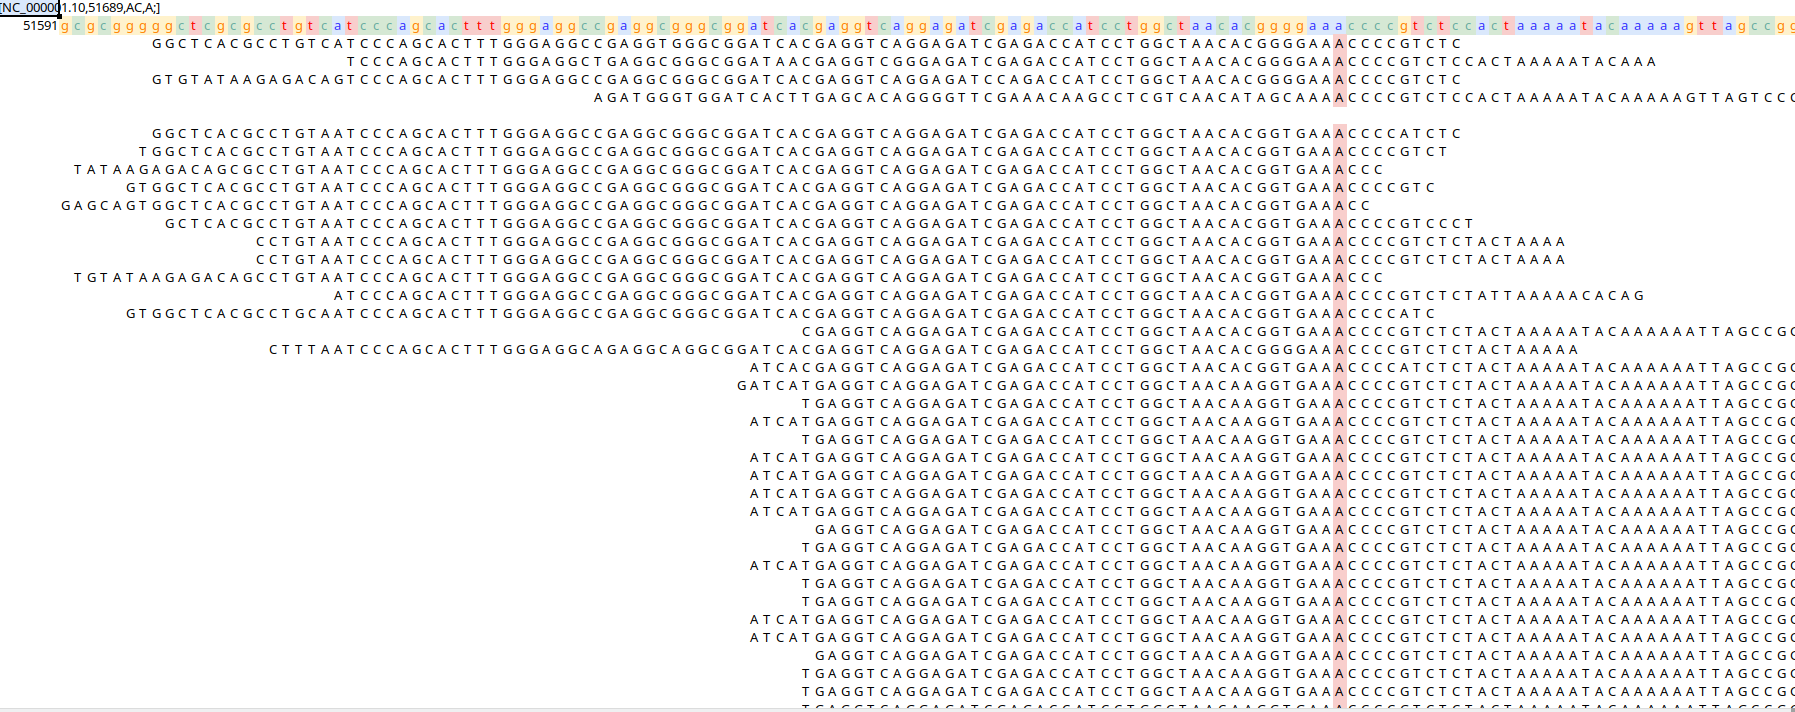
\includegraphics[width=1\columnwidth]{body/image/indel_pileup_ALTread.png}
\caption[Figure 4.22 pileup]{The pileup corresponding to the Figure \ref{indel_new_ALTread} variants.}
\label{indel_pileup_ALTread}
\end{figure}

\begin{figure}[H]
\centering
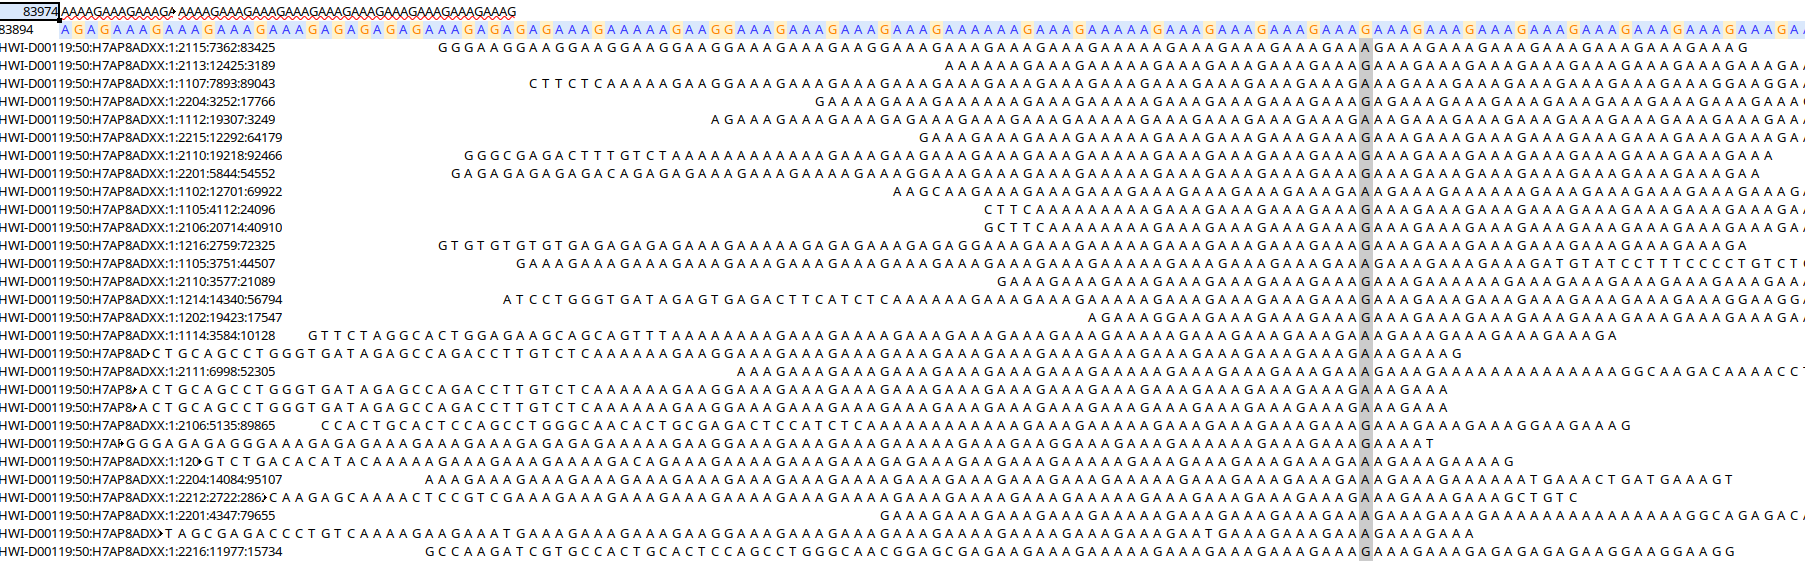
\includegraphics[width=1\columnwidth]{body/image/indel_new_REFread.png}
\caption[INDEL worse match reads]{Matching reads but more similar to reference sequence in INDEL.}
\label{indel_new_REFread}
\end{figure}

\begin{figure}[H]
\centering
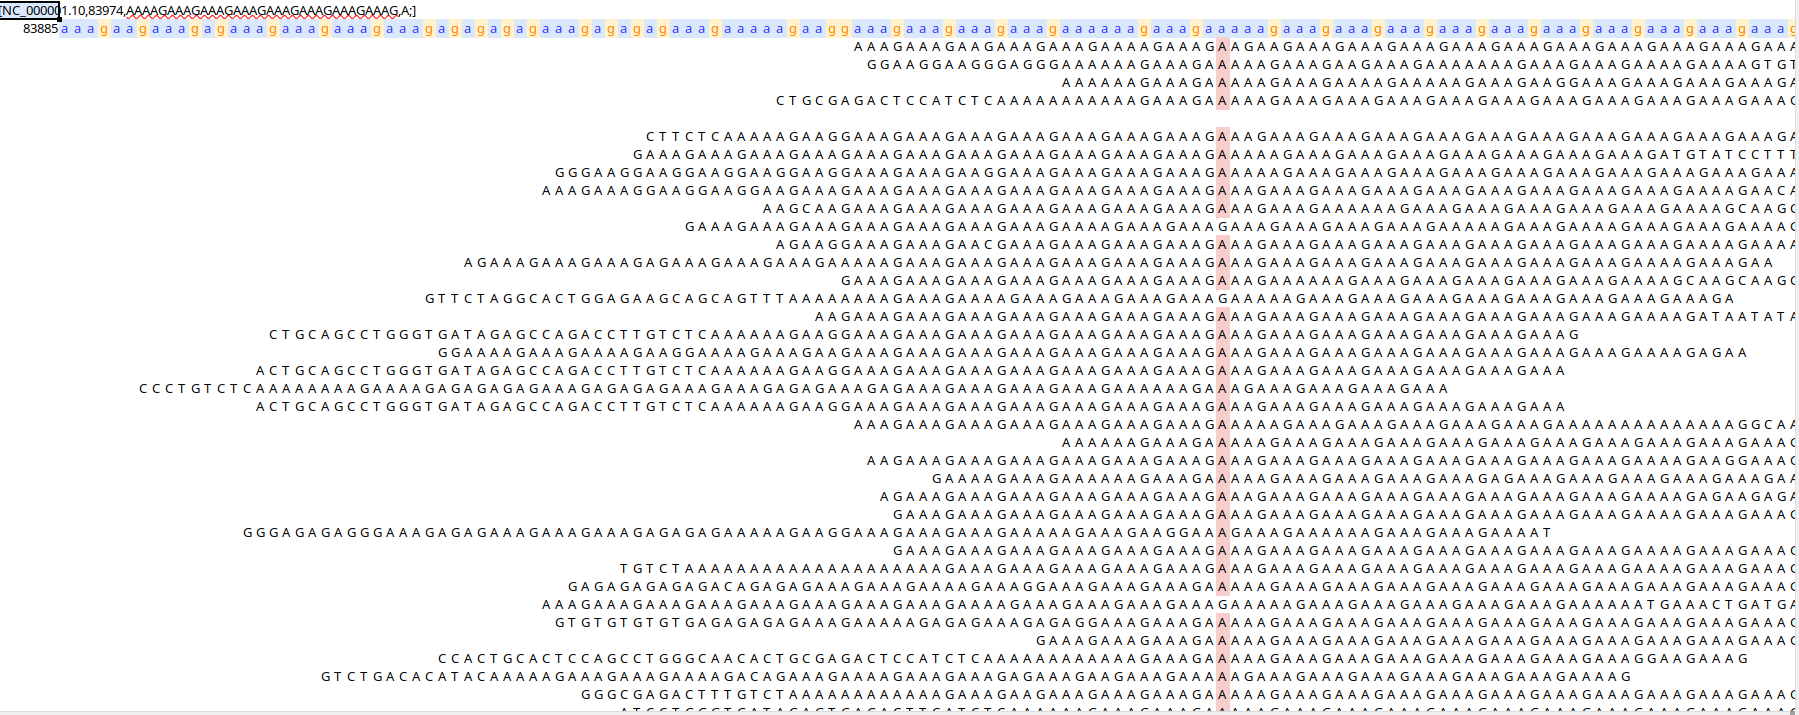
\includegraphics[width=1\columnwidth]{body/image/indel_pileup_REFread.png}
\caption[Figure 4.24 pileup]{The pileup corresponding to the Figure \ref{indel_new_REFread} variants.}
\label{indel_pileup_REFread}
\end{figure}

It can be seen that the reads we found gave EAGLE more evidence for judgment, and that the magnitude of change in INDEL was significantly greater than SNP, just like the experiment we simulated before.

\begin{figure}[H]
\centering
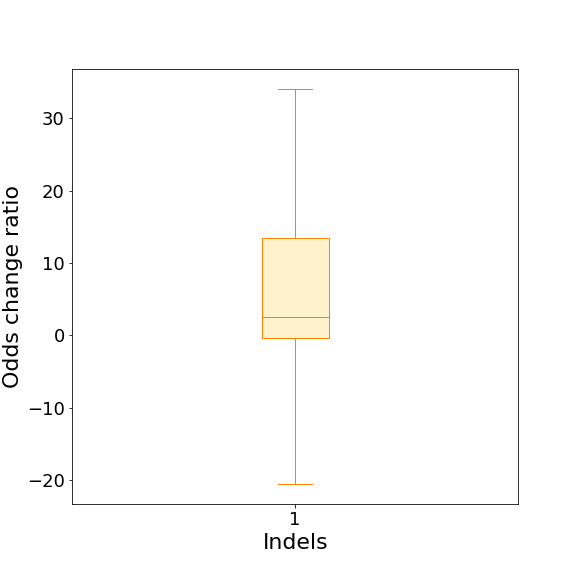
\includegraphics[width=0.6\columnwidth]{body/image/indel_odds_change.png}
\caption[INDEL odds change ratio]{INDEL odds change ratio.}
\label{indel_odds_change}
\end{figure}

\section{Execution time and memory consumption}

Finally, let’s discuss our execution time and memory consumption, our test data are as follows Table\ref{tab:dataset}, test environment as Figure \ref{environment}.

\begin{table}[ht]
    \centering
    \caption[Test Dataset]{Test Dataset}
    \vspace{-0.5cm}
    \resizebox{\textwidth}{25mm}{
    \begin{tabular}{|l|l|l|l|}
    \hline
     &
    \textbf{Reference Genome} &    \textbf{Read} &   \textbf{VCF} \\
    \hline
    \rowcolor{lightgray}
    \textbf{Dataset} &  
    
    \begin{tabular}{p{6cm}}
     Genome Reference Consortium Human Build 37 patch release 13 version
    \end{tabular}
    
    &\begin{tabular}{p{6cm}}
     Garvan NA12878 HG001 HiSeq Exome
    \end{tabular} &
    \begin{tabular}{p{6cm}}
     Single Nucleotide Polymorphism Database (dbSNP)
    \end{tabular} \\
    \hline
    \textbf{File Size} &   3.1G &    5G &  669.7MB \\
    \hline
    \end{tabular}}
    \label{tab:dataset}
\end{table}
\vspace{0.5cm}
\begin{figure}[H]
    \centering
    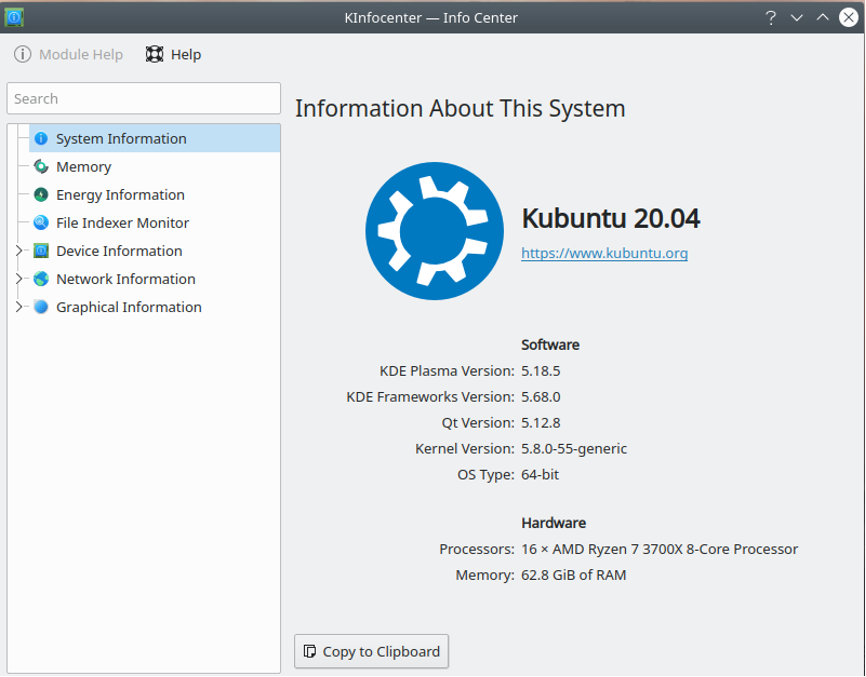
\includegraphics[width=0.8\columnwidth]{body/image/environment.png}
    \captionsetup{labelfont=bf}
    \renewcommand{\baselinestretch}{1.0}
    \caption[Test Environment]{Test Environment.}
    \label{environment}
\end{figure}

Experimenting with the above conditions, first we can see that the memory we consume is 11.64G, and the memory consumed by EAGLE is 0.36G, we can find that the memory space we need is indeed much larger than the original EAGLE. This is because we need to access read-index, reference-index and read files to complete quick searches, so the memory size we need is closely related to these three.
But what we care most about is our execution speed. The time taken by EAGLE is 3618.18 seconds and our method is 6426.28 seconds. Although it seems to take a lot of time, we can find out that we have increased by carefully analyzing our execution time. A large part of the time is to index the read. The time it takes is 1649.33 seconds, but the time to search is very quick, as shown in Figure \ref{search_time}, and a part of the time is because we find more reads, the calculation added by EAGLE Time. Considering this situation, we can say that the added time is relatively small.

\begin{figure}[H]
\centering
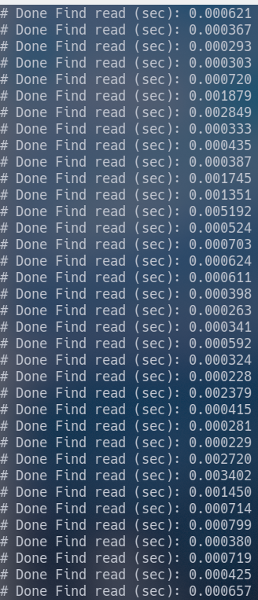
\includegraphics[width=0.4\columnwidth]{body/image/search_time.png}
\caption[searching time]{searching per hypothetical sequence time.}
\label{search_time}
\end{figure}

	
\chapter{Conclusions and Future Work} \label{ch:5-conclusion}
	\hspace{24pt}

\section{Conclusion}
In order to try to reduce the influence of reference bias and improve the accuracy of EAGLE for evaluating variants, we have expanded the function of EAGLE. Before EAGLE calculation, by generating hypothetical sequences that binding variants and reference sequences, and create a read-index to achieve quick search, find out those misalignment or incorrect reads, and finally add it to pileup.

After this series of steps, we conducted an experiment that simulates the real situation to verify our method. The experimental results of our simulation show that our method can effectively reduce the influence of reference bias, and in a longer indel The effect is particularly significant. At the same time, we can work normally in any read coverage situation.

We are also testing in the real data set dbSNP, we can get the same good results as before, but the effect on SNPs is relatively limited.The reason why the method we implemented can be successfully applied to EAGLE is mainly because the EAGLE probability model is mainly used read to estimate the likelihood of each variant, and we can find many reads that are affected by reference bias and are discarded. We only need to increase the establishment of read-index and a little search time to eliminate the influence of reference bias.

\section{Future Work}
In future research, I think we can think about how to establish a more perfect hypothetical sequence. At present, our method is to establish our hypothetical sequence for a single mutation, but we have found that adjacent mutations are prone to occur. Maybe we can consider neighboring variants. Different permutations and combinations generate hypothesis sequences to improve the effect of our method, but it may consume a lot of time.

The possibility of combining good alignment tools by creating better hypotheses is worthy of further investigation.


%====================
%  Back Pages // cbj
%  1. 參考文獻 2. 附錄 3. 作者簡歷
%====================
%%% 參考文獻
\newpage
\phantomsection % for hyperref to register this
\addcontentsline{toc}{chapter}{References}
\renewcommand{\bibname}{\protect\makebox[5cm][s]{REFERENCES}}
%  \makebox{} is fragile; need protect
\bibliographystyle{unsrt}
%\bibliographystyle{IEEEtranS}  % 使用 IEEE Trans 期刊格式
%  \bibliography{my_bib}

%% References with bibTeX database:
%\bibliographystyle{model1-num-names}
\bibliography{back/ncku_thesis_bib}
\baselineskip=18pt
%%\begin{thebibliography}{29}
%%\expandafter\ifx\csname natexlab\endcsname\relax\def\natexlab#1{#1}\fi
%%\providecommand{\bibinfo}[2]{#2}
%%\ifx\xfnm\relax \def\xfnm[#1]{\unskip,\space#1}\fi
%%%Type = Article
%%\bibitem[{Wiegand et~al.(2003)Wiegand, Sullivan, Bjontegaard, and Luthra}]{Wiegand2003}
%%\bibinfo{author}{T.~Wiegand}, \bibinfo{author}{G.~J. Sullivan}, \bibinfo{author}{G.~Bjontegaard}, \bibinfo{author}{A.~Luthra},
%%\newblock \bibinfo{title}{{Overview of the {H.264/AVC} video coding standard}},
%%\newblock \bibinfo{journal}{{\it IEEE Transactions on Circuits and Systems for Video Technology}},
%%\bibinfo{volume}{{\it 13}}(\bibinfo{issue}{7}), \bibinfo{year}{2003}, \bibinfo{pages}{560--576}.
%%%Type = Article
%%\bibitem[{Ostermann et~al.(2004)Ostermann, Bormans, List, Marpe, Narroschke,
%%  Pereira, Stockhammer, and Wedi}]{Ostermann2004}
%%\bibinfo{author}{J.~Ostermann}, \bibinfo{author}{J.~Bormans},
%%  \bibinfo{author}{P.~List}, \bibinfo{author}{D.~Marpe},
%%  \bibinfo{author}{M.~Narroschke}, \bibinfo{author}{F.~Pereira},
%%  \bibinfo{author}{T.~Stockhammer}, \bibinfo{author}{T.~Wedi},
%%\newblock \bibinfo{title}{{Video coding with {H.264/AVC}: tools, performance,
%%  and complexity}},
%%\newblock \bibinfo{journal}{{\it IEEE Circuits and Systems Magazine}},
%%\bibinfo{volume}{{\it 4}}(\bibinfo{issue}{1}), \bibinfo{year}{2004}, \bibinfo{pages}{7--28}.
%%%Type = Article
%%\bibitem[{Marpe et~al.(2006)Marpe, Wiegand, and Sullivan}]{Marpe2006}
%%\bibinfo{author}{D.~Marpe}, \bibinfo{author}{T.~Wiegand},
%%  \bibinfo{author}{G.~J. Sullivan},
%%\newblock \bibinfo{title}{{The {H.264/MPEG4} advanced video coding standard and its applications}},
%%\newblock \bibinfo{journal}{{\it IEEE Communications Magazine}},
%%\bibinfo{volume}{{\it 44}}(\bibinfo{issue}{8}), \bibinfo{year}{2006}, \bibinfo{pages}{134--143}.
%%%Type = Article
%%\bibitem[{Huang et~al.(2005)Huang, Hsieh, Chen, and Chen}]{Huang2005}
%%\bibinfo{author}{Y.-W. Huang}, \bibinfo{author}{B.-Y. Hsieh},
%%\bibinfo{author}{T.-C. Chen}, \bibinfo{author}{L.-G. Chen},
%%\newblock \bibinfo{title}{{Analysis, fast algorithm, and VLSI architecture
%%  design for {H.264/AVC} intra frame coder}},
%%\newblock \bibinfo{journal}{{\it IEEE Transactions on Circuits and Systems for Video Technology}},
%%\bibinfo{volume}{{\it 15}}(\bibinfo{issue}{3}), \bibinfo{year}{2005}, \bibinfo{pages}{378--401}.
%%%Type = Inproceedings
%%\bibitem[{Yu(2004)}]{Yu2004}
%%\bibinfo{author}{A.~C. Yu},
%%\newblock \bibinfo{title}{{Efficient block-size selection algorithm for
%%  inter-frame coding in {H.264/MPEG-4 AVC}}},
%%\newblock \bibinfo{booktitle}{{\it Proc. IEEE Conf. on
%%  Acoustics, Speech, and Signal Processing (ICASSP2004)}}, Montreal, QC, CA, \bibinfo{year}{2004}, \bibinfo{pages}{iii--169--72}.
%%%Type = Article
%%\bibitem[{Wu et~al.(2005)Wu, Pan, Lim, Wu, Li, Lin, Rahardja, and Ko}]{Wu2005}
%%\bibinfo{author}{D.~Wu}, \bibinfo{author}{F.~Pan}, \bibinfo{author}{K.~P. Lim},
%%  \bibinfo{author}{S.~Wu}, \bibinfo{author}{Z.~G. Li},
%%  \bibinfo{author}{X.~Lin}, \bibinfo{author}{S.~Rahardja},
%%  \bibinfo{author}{C.~C. Ko},
%%\newblock \bibinfo{title}{{Fast intermode decision in {H.264/AVC} video
%%  coding}},
%%\newblock \bibinfo{journal}{{\it IEEE Transactions on Circuits and Systems for Video Technology}},
%%  \bibinfo{volume}{{\it 15}}(\bibinfo{issue}{7}), \bibinfo{year}{2005}, \bibinfo{pages}{953--958}.
%%%Type = Article
%%\bibitem[{Grecos and Yang(2006)}]{Grecos2006}
%%\bibinfo{author}{C.~Grecos}, \bibinfo{author}{M.~Yang},
%%\newblock \bibinfo{title}{{Fast mode prediction for the baseline and main
%%  profiles in the {H.264} video coding standard}},
%%\newblock \bibinfo{journal}{{\it IEEE Transactions on Multimedia}},
%%\bibinfo{volume}{{\it 8}}(\bibinfo{issue}{7}), \bibinfo{year}{2006}, \bibinfo{pages}{1125--1134}.
%%%Type = Article
%%\bibitem[{Kannangara et~al.(2006)Kannangara, Richardson, Bystrom, Solera, Zhao, MacLennan, and Cooney}]{Kannangara2006}
%%\bibinfo{author}{C.~S. Kannangara}, \bibinfo{author}{I.~E.~G. Richardson},
%%  \bibinfo{author}{M.~Bystrom}, \bibinfo{author}{J.~R. Solera},
%%  \bibinfo{author}{Y.~Zhao}, \bibinfo{author}{A.~MacLennan},
%%  \bibinfo{author}{R.~Cooney},
%%\newblock \bibinfo{title}{{Low-complexity skip prediction for {H.264} through
%%  Lagrangian cost estimation}},
%%\newblock \bibinfo{journal}{{\it IEEE Transactions on Circuits and Systems for Video Technology}},
%%  \bibinfo{volume}{{\it 16}}(\bibinfo{issue}{2}), \bibinfo{year}{2006}, \bibinfo{pages}{202--208}.
%%%Type = Article
%%\bibitem[{Bharanitharan et~al.(2008)Bharanitharan, Liu, Yang, and
%%  Tsai}]{Bharanitharan2008}
%%\bibinfo{author}{K.~Bharanitharan}, \bibinfo{author}{B.-D. Liu},
%%  \bibinfo{author}{J.-F. Yang}, \bibinfo{author}{W.-C. Tsai},
%%\newblock \bibinfo{title}{{A low complexity detection of discrete cross
%%  differences for fast {H.264/AVC} intra prediction}},
%%\newblock \bibinfo{journal}{{\it IEEE Transactions on Multimedia}},
%% \bibinfo{volume}{{\it 10}}(\bibinfo{issue}{7}), \bibinfo{year}{2008}, \bibinfo{pages}{1250--1260}.
%%%Type = Article
%%\bibitem[{Lee and Lin(2009)}]{Lee2009}
%%\bibinfo{author}{Y.-M. Lee}, \bibinfo{author}{Y.~Lin},
%%\newblock \bibinfo{title}{{Zero-block mode decision algorithm for {H.264/AVC}}},
%%\newblock \bibinfo{journal}{IEEE Transactions on Image Processing},
%%\bibinfo{volume}{{\it 18}}(\bibinfo{issue}{3}), \bibinfo{year}{2009} \bibinfo{pages}{524--533}.
%%%Type = Article
%%\bibitem[{Zeng et~al.(2009)Zeng, Cai, and Ma}]{Zeng2009}
%%\bibinfo{author}{H.~Zeng}, \bibinfo{author}{C.~Cai}, \bibinfo{author}{K.-K.
%%  Ma},
%%\newblock \bibinfo{title}{{Fast mode decision for {H.264/AVC} based on
%%  macroblock motion activity}},
%%\newblock \bibinfo{journal}{{\it IEEE Transactions on Circuits and Systems for Video Technology}},
%%  \bibinfo{volume}{{\it 19}}(\bibinfo{issue}{4}), \bibinfo{year}{2009}, \bibinfo{pages}{491--499}.
%%%Type = Article
%%\bibitem[{Moon et~al.(2005)Moon, Kim, and Kim}]{Moon2005}
%%\bibinfo{author}{Y.~H. Moon}, \bibinfo{author}{G.~Y. Kim},
%%  \bibinfo{author}{J.~H. Kim},
%%\newblock \bibinfo{title}{{An improved early detection algorithm for all-zero
%%  blocks in {H.264} video encoding}},
%%\newblock \bibinfo{journal}{{\it IEEE Transactions on Circuits and Systems for Video Technology}},
%%  \bibinfo{volume}{{\it 15}}(\bibinfo{issue}{8}), \bibinfo{year}{2005}, \bibinfo{pages}{1053--1057}.
%%%Type = Article
%%\bibitem[{Wang et~al.(2006)Wang, Kwong, and Kok}]{Wang2006}
%%\bibinfo{author}{H.~Wang}, \bibinfo{author}{S.~Kwong}, \bibinfo{author}{C.-W. Kok},
%%\newblock \bibinfo{title}{{Efficient prediction algorithm of integer {DCT}
%%  coefficients for {H.264/AVC}optimization}},
%%\newblock \bibinfo{journal}{{\it IEEE Transactions on Circuits and Systems for Video Technology}},
%%  \bibinfo{volume}{{\it 16}}(\bibinfo{issue}{4}), \bibinfo{year}{2006}, \bibinfo{pages}{547--552}.
%%%Type = Article
%%\bibitem[{Wang and Kwong(2007)}]{Wang2007}
%%\bibinfo{author}{H.~Wang}, \bibinfo{author}{S.~Kwong},
%%\newblock \bibinfo{title}{{Hybrid model to detect zero quantized {DCT}
%%  coefficients in {H.264}}},
%%\newblock \bibinfo{journal}{{\it IEEE Transactions on Multimedia}},
%% \bibinfo{volume}{{\it 9}}(\bibinfo{issue}{4}), \bibinfo{year}{2007}, \bibinfo{pages}{728--735}.
%%%Type = Article
%%\bibitem[{Xie et~al.(2007)Xie, Liu, Liu, and Yang}]{Xie2007}
%%\bibinfo{author}{Z.~Xie}, \bibinfo{author}{Y.~Liu}, \bibinfo{author}{J.~Liu},
%%  \bibinfo{author}{T.~Yang},
%%\newblock \bibinfo{title}{{A general method for detecting all-zero blocks prior
%%  to {DCT} and quantization}},
%%\newblock \bibinfo{journal}{{\it IEEE Transactions on Circuits and Systems for Video Technology}},
%%  \bibinfo{volume}{{\it 17}}(\bibinfo{issue}{2}), \bibinfo{year}{2007}, \bibinfo{pages}{237--241}.
%%%Type = Article
%%\bibitem[{Sousa(2000)}]{Sousa2000}
%%\bibinfo{author}{L.~A. Sousa},
%%\newblock \bibinfo{title}{{General method for eliminating redundant computations in video coding}},
%%\newblock \bibinfo{journal}{{\it Electronics Letters}},
%%\bibinfo{volume}{36}(\bibinfo{issue}{2}), \bibinfo{year}{2000}, \bibinfo{pages}{306--307}.
%%%Type = Article
%%\bibitem[{Pao and Sun(1999)}]{Pao1999}
%%\bibinfo{author}{I.-M. Pao}, \bibinfo{author}{M.-T. Sun},
%%\newblock \bibinfo{title}{{Modeling {DCT} coefficients for fast video
%%  encoding}},
%%\newblock \bibinfo{journal}{{\it IEEE Transactions on Circuits and Systems for Video Technology}},
%%  \bibinfo{volume}{{\it 9}}(\bibinfo{issue}{4}),\bibinfo{year}{1999},\bibinfo{pages}{608--616}.
%%%Type = Manual
%%\bibitem[{Sta(2007)}]{StandardAVC}
%%\bibinfo{title}{{{ITU}-T Recommendation H.264 : Advanced video coding for
%%  generic audiovisual services}}, \bibinfo{organization}{International
%%  Telecommunications Union}, \bibinfo{year}{2007}.
%%%Type = Book
%%\bibitem[{Richardson(2003)}]{Richardson2003}
%%\bibinfo{author}{I.~Richardson}, \bibinfo{title}{{\it H.264 and MPEG-4 video
%%  compression: video coding for next-generation multimedia}},
%%  (\bibinfo{publisher}{Wiley}, \bibinfo{year}{2003}).
%%%Type = Article
%%\bibitem[{Lam and Goodman(2000)}]{Lam2000}
%%\bibinfo{author}{E.~Y. Lam}, \bibinfo{author}{J.~W. Goodman},
%%\newblock \bibinfo{title}{{A mathematical analysis of the DCT coefficient
%%  distributions for images}},
%%\newblock \bibinfo{journal}{{\it IEEE Transactions on Image Processing}},
%% \bibinfo{volume}{{\it 9}}(\bibinfo{issue}{10}), \bibinfo{year}{2000}, \bibinfo{pages}{1661--1666}.
%%%Type = Article
%%\bibitem[{Reininger(1983)}]{Reininger1983}
%%\bibinfo{author}{R.~Reininger} \& \bibinfo{author}{J.~Gibson},
%%\newblock \bibinfo{title}{{Distribution of the two dimensional dct coefficients
%%  for images}},
%%\newblock \bibinfo{journal}{{\it IEEE Transactions on Communications}},
%% \bibinfo{volume}{{\it 31}}(\bibinfo{issue}{6}), \bibinfo{year}{1983}, \bibinfo{pages}{835--839}.
%%%Type = Inproceedings
%%\bibitem[{Altunbasak and Kamaci(2004)}]{Altunbasak2004}
%%\bibinfo{author}{Y.~Altunbasak}, \bibinfo{author}{N.~Kamaci},
%%\newblock \bibinfo{title}{{An analysis of the DCT coefficient distribution with
%%  the H.264 video coder}},
%%\newblock \bibinfo{booktitle}{{\it Proc. IEEE Conf. on Acoustics, Speech, and Signal Processing (ICASSP2004)}}, Montreal, QC, CA, \bibinfo{year}{2004},
%%\bibinfo{pages}{iii --177--80}.
%%%Type = Book
%%\bibitem[{Eude et~al.(1994{\natexlab{a}})Eude, Cherifi, and Grisel}]{Eude1994a}
%%\bibinfo{author}{T.~Eude}, \bibinfo{author}{H.~Cherifi},
%%  \bibinfo{author}{R.~Grisel}, \bibinfo{title}{{Statistical distribution of DCT
%%  coefficients and their application to an adaptive compression algorithm}},
%%  \newblock \bibinfo{booktitle}{{\it IEEE Region 10 Conf. (TENCON1994)}}, \bibinfo{year}{1994}, Singapore, Singapore, \bibinfo{pages}{427--430}.
%%%Type = Inproceedings
%%\bibitem[{Eude et~al.(1994{\natexlab{b}})Eude, Grisel, Cherifi, and
%%  Debrie}]{Eude1994b}
%%\bibinfo{author}{T.~Eude}, \bibinfo{author}{R.~Grisel},
%%  \bibinfo{author}{H.~Cherifi}, \bibinfo{author}{R.~Debrie},
%%\newblock \bibinfo{title}{{On the distribution of the DCT coefficients}},
%%\newblock \bibinfo{booktitle}{{\it Proc. IEEE Conf. on Acoustics, Speech, and Signal Processing (ICASSP1994)}},
%%  \bibinfo{year}{1994}, Adelaide, SA, AU, \bibinfo{pages}{v--365--368}.
%%%Type = Article
%%\bibitem[{Xie and Chia(2008)}]{Xie2008}
%%\bibinfo{author}{J.~Xie}, \bibinfo{author}{L.-T. Chia},
%%\newblock \bibinfo{title}{{\it Study on the distribution of DCT residues and its
%%  application to R-D analysis of video coding}},
%%\newblock \bibinfo{journal}{Journal of Visual Communication and Image Representation},
%% \bibinfo{volume}{19}(\bibinfo{issue}{7}), \bibinfo{year}{2008}, \bibinfo{pages}{411--425}.
%%%Type = Book
%%\bibitem[{Jain(1989)}]{Jain1989}
%%\bibinfo{author}{A.~Jain}, \bibinfo{title}{{\it Fundamentals of digital image
%%  processing}} (\bibinfo{publisher}{Inc. Upper Saddle River, NJ:Prentice-Hall}, \bibinfo{year}{1989}).
%%%Type = Article
%%\bibitem[{Hang and Chen(1997)}]{Hang1997}
%%\bibinfo{author}{H.-M. Hang}, \bibinfo{author}{J.-J. Chen},
%%\newblock \bibinfo{title}{{Source model for transform video coder and its
%%  application - Part I: Fundamental theory}},
%%\newblock \bibinfo{journal}{{\it IEEE Transactions on Circuits and Systems for Video Technology}},
%% \bibinfo{volume}{{\it 7}}(\bibinfo{issue}{2}), \bibinfo{year}{1997}, \bibinfo{pages}{287--298}.
%%%Type = Article
%%\bibitem[{Ma(2005)}]{Ma2005}
%%\bibinfo{author}{S.~Ma},
%%\newblock \bibinfo{title}{{Rate-distortion analysis for H.264/AVC video coding
%%  and its application to rate control}},
%%\newblock \bibinfo{journal}{{\it IEEE Transactions on Circuits and Systems for Video Technology}},
%% \bibinfo{volume}{{\it 15}}(\bibinfo{issue}{12}), \bibinfo{year}{2005}, \bibinfo{pages}{1533--1544}.
%%%Type = Manual
%%\bibitem[{JMS(2008)}]{JMSoftware}
%%\bibinfo{title}{{{H.264/AVC} reference software, Joint Model (JM), [{O}nline]. Available:
%%  http://iphome.hhi.de/suehring/tml/}}.

%%\end{thebibliography}


%%% 附錄
%%
% this file is encoded in utf-8
% v2.0 (Apr. 5, 2009)
%%% 每一個附錄 (附錄甲、附錄乙、...) 都要複製此段附錄編排碼做為起頭
%%% 附錄編排碼 begin >>>
\newpage
\chapter*{Appendix A: MATLAB / Octave } % 修改附錄編號與你的附錄名
\phantomsection % for hyperref to register this
\addcontentsline{toc}{chapter}{Appendix A: MATLAB / Octave} %建議此內容應與上行相同
%\setcounter{chapter}{0}  %如果用的是 TeXLive2007 則打開此行以避免錯誤
\setcounter{equation}{0} 
\setcounter{figure}{0} 
\setcounter{footnote}{0} 
\setcounter{section}{0} 
\setcounter{subsection}{0}
\setcounter{subsubsection}{0}
\setcounter{table}{0} 
\renewcommand{\thechapter}{A} % 如果是附錄乙,則內容應為{乙}
%%% <<< 附錄編排碼 end

% 附錄內容開始
% 納入程式源碼
%\lstinputlisting{example_prog_list.m}


\begin{equation}\sum_{k=1}^{n} k = \frac{n(n+1)}{2}\end{equation}

%%% 如果有附錄乙、丙、...,則在此繼續加上「附錄編排」碼
% 每一個附錄會自動以新頁開始
%%% 自傳
%\newpage
\chapter*{\nameVita} % \makebox{} is fragile; need protect
\phantomsection % for hyperref to register this
\addcontentsline{toc}{chapter}{\nameVitac}

\noindent
{\it Bo-Jhih Chen} received his B.S. and M.S. degree in I-Shou University, Kaohsiung, Taiwan (R.O.C.), in 2004 and 2006, respectively. He got his Ph.D. degree of the Institute of Computer and Communication Engineering at Department of Electrical Engineering in National Cheng Kung University, Tainan, Taiwan (R.O.C.), in 2012.
His research interests are in the areas of video coding standards, digital signal processing, and multimedia system.
\bigskip \\
\noindent {\bf Education Background}\\
\noindent Sept. 2006 -- June 2012:\\
	Ph.D., Institute of Computer and Communication Engineering, Department of Electrical Engineering, National Cheng Kung University.\\
\noindent Sept. 2004 -- June 2006:\\
	M.S., Department of Computer Science and Information Engineering, I-Shou University.\\
\noindent Sept. 2000 -- June 2004:\\
	B.S., Department of Computer Science and Information Engineering, I-Shou University.

\end{document}
